\documentclass[11pt]{article}%
\usepackage{geometry}%
\geometry{a4paper,
  lmargin=2cm,rmargin=2cm,tmargin=2.5cm,bmargin=2.5cm}

\input{../macros_Livre.tex}

% \renewcommand{\thesection}{\Roman{section}.\hspace{-.3cm}}
% \renewcommand{\thesubsection}{\Alph{subsection}.\hspace{-.2cm}}

\pagestyle{fancy} %
\pagestyle{fancy} %
 \lhead{ECE2 \hfill Mathématiques \\} %
\chead{\hrule} %
\rhead{} %
\lfoot{} %
\cfoot{} %
\rfoot{\thepage} %

\renewcommand{\headrulewidth}{0pt}% : Trace un trait de séparation
                                    % de largeur 0,4 point. Mettre 0pt
                                    % pour supprimer le trait.

\renewcommand{\footrulewidth}{0.4pt}% : Trace un trait de séparation
                                    % de largeur 0,4 point. Mettre 0pt
                                    % pour supprimer le trait.

\setlength{\headheight}{14pt}

\title{\bf \vspace{-1.6cm} EML 2016} %
\author{} %
\date{} %
\begin{document}

\maketitle %
\vspace{-1.2cm}\hrule %
\thispagestyle{fancy}

\vspace*{.4cm}

%%DEBUT

\section*{EXERCICE I}

\noindent
On note $I$ et $A$ les matrices de $\M{3}$ définies 
par :
\[
I=
\begin{smatrix}
 1 & 0 & 0\\
 0 & 1 & 0\\
 0 & 0 & 1
\end{smatrix}
, \qquad 
A=
\begin{smatrix}
 0 & 1 & 0\\
 1 & 0 & 1\\
 0 & 1 & 0
\end{smatrix},
\]
et $\mathcal{E}$ l'ensemble des matrices de $\M{3}$ 
défini par :
\[
\mathcal{E}=\left\{
\begin{smatrix}
 a+c & b & c\\
 b & a+2c & b\\
 c & b & a+c
\end{smatrix} \; ; \; (a,b,c) \in \R^3 \right\}
\]

\subsection*{PARTIE I : Étude de la matrice $A$}

\begin{noliste}{1.}
\setlength{\itemsep}{2mm}
\item Calculer $A^2$.

\begin{proof}~
 \[
  A^2=
  \begin{smatrix}
   0 & 1 & 0\\
   1 & 0 & 1\\
   0 & 1 & 0
  \end{smatrix}
  \times
  \begin{smatrix}
   0 & 1 & 0\\
   1 & 0 & 1\\
   0 & 1 & 0
  \end{smatrix}
  =
  \begin{smatrix}
   1 & 0 & 1\\
   0 & 2 & 0\\
   1 & 0 & 1
  \end{smatrix}
 \]
 \conc{$A^2=
 \begin{smatrix}
   1 & 0 & 1\\
   0 & 2 & 0\\
   1 & 0 & 1
  \end{smatrix}$}~\\[-1cm]
\end{proof}


\item Montrer que la famille $(I,A,A^2)$ est libre.

\begin{proof}~\\
 Soit $(\lambda_1, \lambda_2,\lambda_3)\in\R^3$. On suppose :
 \[
  \lambda_1 \cdot I_3 + \lambda_2 \cdot A + \lambda_3 \cdot A^2 
  =0_{\M{3}} \qquad (1)
 \]
 Or :
 \[
  \begin{array}{rcl}
   \lambda_1 \cdot I_3 + \lambda_2 \cdot A + \lambda_3 \cdot A^2 &=&
   \lambda_1 \cdot
   \begin{smatrix}
    1 & 0 & 0\\
    0 & 1 & 0\\
    0 & 0 & 1
   \end{smatrix}
   + \lambda_2 \cdot
   \begin{smatrix}
    0 & 1 & 0\\
    1 & 0 & 1\\
    0 & 1 & 0
   \end{smatrix}
   + \lambda_3 \cdot
   \begin{smatrix}
    1 & 0 & 1\\
    0 & 2 & 0\\
    1 & 0 & 1
   \end{smatrix}
   \\[.8cm]
   &=& 
   \begin{smatrix}
    \lambda_1 + \lambda_3 & \lambda_2 & \lambda_3\\
    \lambda_2 & \lambda_1 + 2 \lambda_3 & \lambda_2\\
    \lambda_3 & \lambda_2 & \lambda_1 + \lambda_3
   \end{smatrix}
  \end{array}
 \]
 L'égalité $(1)$ entraîne alors :
 \[
  \begin{array}{rcl}
   \left\{
   \begin{array}{rrrrrcl}
    \lambda_1 & & & + & \lambda_3 & = & 0\\
    \lambda_1 & & & + & 2\, \lambda_3 & = & 0\\
    & & \lambda_2 & & & = & 0\\
    & & & & \lambda_3 & = & 0
   \end{array}
   \right.
   & \Leftrightarrow &
   \left\{
    \lambda_1 = 
    \lambda_2 = 
    \lambda_3 = 0
   \right.
   \\[-.6cm]
   & & \mbox{\it{(par remontées successives)}}
  \end{array}
 \]
 
\conc{La famille $(I,A,A^2)$ est libre.}~\\[-1.2cm] 
\end{proof}

%\newpage

\item
\begin{noliste}{a)}
\item Justifier, sans calcul, que $A$ est diagonalisable.

\begin{proof}~
 \conc{$A$ est une matrice symétrique réelle, donc elle est 
 diagonalisable.}~\\[-1.2cm]
\end{proof}

\item Déterminer une matrice $P$ de $\M{3}$ 
inversible dont tous les coefficients de la première ligne sont égaux à 
1 et une matrice $D$ de $\M{3}$ diagonale dont tous 
les coefficients diagonaux sont dans l'ordre croissant telles que : 
$A=PDP^{-1}$.

\begin{proof}~
 \begin{noliste}{$\sbullet$}
  \item D'après la question \itbf{3.a)}, la matrice $A$ est 
  diagonalisable. Donc il existe une matrice $P$ inversible 
  ($P$ est la concaténation des vecteurs des 
  bases des sous-espaces propres de $A$) et une matrice $D$ diagonale 
  dont les coefficients diagonaux sont les valeurs propres de $A$ 
  telles que $A=PDP^{-1}$.
  \item Déterminons les valeurs propres de $A$.\\
  Les valeurs propres de $A$ sont les réels $\lambda$ tels que la 
  matrice $(A-\lambda I)$ n'est pas inversible, c'est-à-dire 
  $\rg(A-\lambda 
  I)<3$.\\
  Soit $\lambda\in\R$.
  \[
	 \begin{array}{rcl}
	  \rg(A-\lambda I) &=& \rg\left(
	  \begin{smatrix}
	   -\lambda & 1 & 0\\
	   1 & -\lambda & 1\\
	   0 & 1 & -\lambda
	  \end{smatrix}\right)
	  \\[.8cm]
	  &
	  \begin{arrayEg}
	   L_1 \leftrightarrow L_2
	  \end{arrayEg}
	  &
	  \rg\left(
	  \begin{smatrix}
	   1 & -\lambda & 1\\
	   -\lambda & 1 & 0\\
	   0 & 1 & -\lambda
	  \end{smatrix}\right)
	  \\[.8cm]
	  &
	  \begin{arrayEg}
	   L_2 \leftarrow L_2+\lambda L_1
	  \end{arrayEg}
	  &
	  \rg\left(
	  \begin{smatrix}
	   1 & -\lambda & 1\\
	   0 & 1-\lambda^2 & \lambda\\
	   0 & 1 & -\lambda
	  \end{smatrix}\right)
	  \\[.8cm]
	  &
	  \begin{arrayEg}
	   L_2 \leftrightarrow L_3
	  \end{arrayEg}
	  &
	  \rg\left(
	  \begin{smatrix}
	   1 & -\lambda & 1\\
	   0 & 1 & -\lambda\\
	   0 & 1-\lambda^2 & \lambda
	  \end{smatrix}\right)
	  \\[.8cm]
	  &
	  \begin{arrayEg}
	   L_3 \leftarrow L_3 - (1-\lambda^2)L_2
	  \end{arrayEg}
	  &
	  \rg\left(
	  \begin{smatrix}
	   1 & -\lambda & 1\\
	   0 & 1 & -\lambda\\
	   0 & 0 & \lambda+\lambda(1-\lambda^2)
	  \end{smatrix}\right)
	 \end{array}
	\]
	On obtient une réduite triangulaire supérieure.\\ 
	Elle est donc non inversible si et seulement si l'un de ses 
	coefficients diagonaux est nul.\\ 
	Ses $2$ premiers coefficients diagonaux sont $1$ et $1$ (et 
	$1\neq 0$), et on a :
	  \[
	    \lambda+\lambda(1+\lambda^2)=0 \ \Leftrightarrow \ \lambda 
	    (2-\lambda^2)=0 \ \Leftrightarrow \ 
	    \lambda(\sqrt{2}-\lambda)(\sqrt{2}+\lambda)=0
	    \ \Leftrightarrow \
	    \lambda\in\{0,-\sqrt{2},\sqrt{2}\}
	  \]
	  Ainsi : $\rg(A-\lambda I)<3 \ \Leftrightarrow \ 
	  \lambda\in\{0,-\sqrt{2},\sqrt{2}\}$.\\
	  \conc{Las valeurs propres de $A$ sont $-\sqrt{2}$, $0$ et 
	  $\sqrt{2}$.}
	  
	  %\newpage
	  
  \item Déterminons une base de $E_{\sqrt{2}}(A)$ le sous-espace 
  propre de $A$ associé à la valeur propre $\sqrt{2}$.\\
  Soit $X=
	\begin{smatrix}
	 x\\ y\\ z
	\end{smatrix}\in\M{3,1}$.
	\[
	 \begin{array}{rcl}
	  X\in E_{\sqrt{2}}(A)
	  & \Longleftrightarrow & (A-\sqrt{2}\, I)X=0
	  \\[.2cm]
	  & \Longleftrightarrow & 
	  \begin{smatrix}
	   -\sqrt{2} & 1 & 0\\
	   1 & -\sqrt{2} & 1\\
	   0 & 1 & -\sqrt{2}
	  \end{smatrix}
	  \begin{smatrix}
	   x\\ y\\ z
	  \end{smatrix}
	  =
	  \begin{smatrix}
	   0\\ 0\\ 0
	  \end{smatrix}
	  \\[.8cm]
	  & \Longleftrightarrow & 
	  \left\{
	  \begin{array}{rrrrrcl}
	   -\sqrt{2}\, x & + & y & & & = & 0\\
	   x & - & \sqrt{2}\, y & + & z & = & 0\\
	    & & y & - & \sqrt{2}\, z & = & 0
	  \end{array}
	  \right.
	  \\[.8cm]
	  &
	  \begin{arrayEq}
	   L_1 \leftrightarrow L_2
	  \end{arrayEq}
	  &
	  \left\{
	  \begin{array}{rrrrrcl}
	   x & - & \sqrt{2}\, y & + & z & = & 0\\
	   -\sqrt{2}\, x & + & y & & & = & 0\\
	    & & y & - & \sqrt{2}\, z & = & 0
	  \end{array}
	  \right.
	  \\[.8cm]
	  &
	  \begin{arrayEq}
	   L_2 \leftarrow L_2+\sqrt{2}\, L_1
	  \end{arrayEq}
	  &
	  \left\{
	  \begin{array}{rrrrrcl}
	   x & - & \sqrt{2} \, y & + & z & = & 0\\
	    & - & y & + & \sqrt{2} \, z & = & 0\\
	    & & y & - & \sqrt{2} \, z & = & 0
	  \end{array}
	  \right.
	  \\[.8cm]
	  &
	  \Longleftrightarrow
	  &
	  \left\{
	  \begin{array}{rrrrrcl}
	   x & - & \sqrt{2} \, y & + & z & = & 0\\
	    & & y & - & \sqrt{2} \, z & = & 0
	  \end{array}
	  \right.
	  \\[.8cm]
	  &
	  \Longleftrightarrow
	  &
	  \left\{
	  \begin{array}{rrrcl}
	   x & - & \sqrt{2} \, y & = & -z\\
	    & & y & = & \sqrt{2} \, z
	  \end{array}
	  \right.
	  \\[.8cm]
	  &
	  \begin{arrayEq}
	   L_1 \leftarrow L_1+\sqrt{2} \, L_2
	  \end{arrayEq}
	  &
	  \left\{
	  \begin{array}{rcl}
	   x & = & -z+2z=z\\
	   y & = & \sqrt{2} \, z
	  \end{array}
	  \right.
	 \end{array}
	\]
	
	Finalement on obtient l'expression de $E_{\sqrt{2}}(A)$ 
	suivante :
	\[
	 \begin{array}{rcl}
	  E_{\sqrt{2}}(A) & = & \{X\in\M{3,1} \ | \ AX=\sqrt{2}\, X\}
	   = \{
	  \begin{smatrix}
	   x\\ y\\ z
	  \end{smatrix}
	  \ | \
	   x = z \mbox{ et }
	   y = \sqrt{2} \, z
	  \}
	  \\[.6cm]
	  & = & \left\{\right.
	  \begin{smatrix}
	   z\\ 
	   \sqrt{2}\, z\\ 
	   z
	  \end{smatrix}
	  \ \left/ \
	  z\in\R\right\}
	   = \left\{\right. z \cdot
	  \begin{smatrix}
	   1\\ 
	   \sqrt{2}\\ 
	   1
	  \end{smatrix}
	  \ \left/ \
	  z\in\R\right\}
	  \\[.6cm]
	  & = & \Vect{
	  \begin{smatrix}
	   1\\ \sqrt{2}\\ 1
	  \end{smatrix}
	  }
	 \end{array}
	\]
	On sait donc que la famille $\left( \begin{smatrix}
	   1\\ \sqrt{2}\\ 1
	  \end{smatrix}\right)$ :
	\begin{noliste}{$\stimes$}
	  \item engendre $E_{\sqrt{2}}(A)$,
	  \item est une famille libre de $\M{3,1}$ car elle est 
	  constituée d'un unique vecteur non nul.
	\end{noliste}
	
	\conc{$\left( \begin{smatrix}
	   1\\ \sqrt{2}\\ 1
	  \end{smatrix}\right)$ est une base de $E_{\sqrt{2}}(A)$.}
	  
  \item Déterminons une base de $E_{0}(A)$ le sous-espace 
  propre de $A$ associé à la valeur propre $0$.\\
  Soit $X=
	\begin{smatrix}
	 x\\ y\\ z
	\end{smatrix}\in\M{3,1}$.
	\[
	 \begin{array}{rcl}
	  X\in E_{0}(A) & \Longleftrightarrow & AX=0
	  \\[.2cm]
	  & \Longleftrightarrow & 
	  \begin{smatrix}
	   0 & 1 & 0\\
	   1 & 0 & 1\\
	   0 & 1 & 0
	  \end{smatrix}
	  \begin{smatrix}
	   x\\ y\\ z
	  \end{smatrix}
	  =
	  \begin{smatrix}
	   0\\ 0\\ 0
	  \end{smatrix}
	  \\[.8cm]
	  & \Longleftrightarrow & 
	  \left\{
	  \begin{array}{rrrrrcl}
	    & & y & & & = & 0\\
	   x & & & + & z & = & 0\\
	    & & y & & & = & 0
	  \end{array}
	  \right.
	  \\[.8cm]
	  &
	  \Longleftrightarrow
	  &
	  \left\{
	  \begin{array}{rrrrrcl}
	   x & & & + & z & = & 0\\
	    & & y & & & = & 0
	  \end{array}
	  \right.
	  \\[.8cm]
	  &
	  \Longleftrightarrow
	  &
	  \left\{
	  \begin{array}{rrrcl}
	   x & & & = & -z\\
	   & & y & = & 0
	  \end{array}
	  \right.
	 \end{array}
	\]
	Finalement on obtient l'expression de $E_{0}(A)$ suivante :
	\[
	 \begin{array}{rcl}
	  E_{0}(A) & = & \{X\in\M{3,1} \ | \ AX=0\}
	  = \{
	  \begin{smatrix}
	   x\\ y\\ z
	  \end{smatrix}
	  \ | \
	   x = -z \mbox{ et }
	   y = 0
	  \}
	  \\[.6cm]
	  & = & \left\{\right.
	  \begin{smatrix}
	   x\\ 0\\ -x
	  \end{smatrix}
	  \ \left/ \
	  x\in\R\right\}
	  = \left\{\right. x \cdot
	  \begin{smatrix}
	   1\\ 0\\ -1
	  \end{smatrix}
	  \ \left/ \
	  x\in\R\right\}
	  \\[.6cm]
	  & = & \Vect{
	  \begin{smatrix}
	   1\\ 0\\ -1
	  \end{smatrix}
	  }
	 \end{array}
	\]
	On sait donc que la famille $\left( \begin{smatrix}
	   1\\ 0\\ -1
	  \end{smatrix}\right)$ :
	\begin{noliste}{$\stimes$}
	  \item engendre $E_{0}(A)$,
	  \item est une famille libre de $\M{3,1}$ car elle est 
	  constituée d'un unique vecteur non nul.
	\end{noliste}
	
	\conc{$\left( \begin{smatrix}
	   1\\ 0\\ -1
	  \end{smatrix}\right)$ est une base de $E_{0}(A)$.}
	  
	  %\newpage
  
  \item Déterminons une base de $E_{-\sqrt{2}}(A)$ le sous-espace 
  propre de $A$ associé à la valeur propre $-\sqrt{2}$.\\
  Soit $X=
	\begin{smatrix}
	 x\\ y\\ z
	\end{smatrix}\in\M{3,1}$.
	\[
	 \begin{array}{rcl}
	  X\in E_{-\sqrt{2}}(A) 
	  & \Longleftrightarrow & (A+\sqrt{2}\, I)X=0
	  \\[.2cm]
	  & \Longleftrightarrow & 
	  \begin{smatrix}
	   \sqrt{2} & 1 & 0\\
	   1 & \sqrt{2} & 1\\
	   0 & 1 & \sqrt{2}
	  \end{smatrix}
	  \begin{smatrix}
	   x\\ y\\ z
	  \end{smatrix}
	  =
	  \begin{smatrix}
	   0\\ 0\\ 0
	  \end{smatrix}
	  \\[.8cm]
	  & \Longleftrightarrow & 
	  \left\{
	  \begin{array}{rrrrrcl}
	   \sqrt{2}\, x & + & y & & & = & 0\\
	   x & + & \sqrt{2}\, y & + & z & = & 0\\
	    & & y & + & \sqrt{2}\, z & = & 0
	  \end{array}
	  \right.
	  \\[.8cm]
	  &
	  \begin{arrayEq}
	   L_1 \leftrightarrow L_2
	  \end{arrayEq}
	  &
	  \left\{
	  \begin{array}{rrrrrcl}
	   x & + & \sqrt{2}\, y & + & z & = & 0\\
	   \sqrt{2}\, x & + & y & & & = & 0\\
	    & & y & + & \sqrt{2}\, z & = & 0
	  \end{array}
	  \right.
	  \\[.8cm]
	  &
	  \begin{arrayEq}
	   L_2 \leftarrow L_2-\sqrt{2}\, L_1
	  \end{arrayEq}
	  &
	  \left\{
	  \begin{array}{rrrrrcl}
	   x & + & \sqrt{2}\, y & + & z & = & 0\\
	    & - & y & - & \sqrt{2}\, z & = & 0\\
	    & & y & + & \sqrt{2}\, z & = & 0
	  \end{array}
	  \right.
	  \\[.8cm]
	  &
	  \Longleftrightarrow
	  &
	  \left\{
	  \begin{array}{rrrrrcl}
	   x & + & \sqrt{2}\, y & + & z & = & 0\\
	    & & y & + & \sqrt{2}\, z & = & 0
	  \end{array}
	  \right.
	  \\[.8cm]
	  &
	  \Longleftrightarrow
	  &
	  \left\{
	  \begin{array}{rrrcl}
	   x & + & \sqrt{2} \, y & = & -z\\
	    & & y & = & -\sqrt{2} \, z
	  \end{array}
	  \right.
	  \\[.8cm]
	  &
	  \begin{arrayEq}
	   L_1 \leftarrow L_1-\sqrt{2} \, L_2
	  \end{arrayEq}
	  &
	  \left\{
	  \begin{array}{rcl}
	   x & = & -z+2z=z\\
	   y & = & -\sqrt{2} \, z
	  \end{array}
	  \right.
	 \end{array}
	\]
	Finalement on obtient l'expression de $E_{-\sqrt{2}}(A)$ 
	suivante :
	\[
	 \begin{array}{rcl}
	  E_{-\sqrt{2}}(A) & = & \{X\in\M{3,1} \ | \ AX=-\sqrt{2}\, X\}
	  = \{
	  \begin{smatrix}
	   x\\ y\\ z
	  \end{smatrix}
	  \ | \
	   x = z \mbox{ et }
	   y = -\sqrt{2} \, z
	  \}
	  \\[.6cm]
	  & = & \left\{\right.
	  \begin{smatrix}
	   z\\ -\sqrt{2}\, z\\ z
	  \end{smatrix}
	  \ \left/ \
	  z\in\R\right\}
	  = \left\{\right. z \cdot
	  \begin{smatrix}
	   1\\ -\sqrt{2}\\ 1
	  \end{smatrix}
	  \ \left/ \
	  z\in\R\right\}
	  \\[.6cm]
	  & = & \Vect{
	  \begin{smatrix}
	   1\\ -\sqrt{2}\\ 1
	  \end{smatrix}
	  }
	 \end{array}
	\]
	On sait donc que la famille $\left( \begin{smatrix}
	   1\\ -\sqrt{2}\\ 1
	  \end{smatrix}\right)$ :
	\begin{noliste}{$\stimes$}
	  \item engendre $E_{-\sqrt{2}}(A)$, d'après le point précédent,
	  \item est une famille libre de $\M{3,1}$ car elle est 
	  constituée d'un unique vecteur non nul.
	\end{noliste}
	
	\conc{$\left( \begin{smatrix}
	   1\\ -\sqrt{2}\\ 1
	  \end{smatrix}\right)$ est une base de $E_{-\sqrt{2}}(A)$.}
	  
	  %\newpage
	  
  \item On rappelle que la matrice $P$ est la concaténation des
  vecteurs des
  bases des sous-espaces propres de $A$, et la matrice $D$ des 
  valeurs propres de $A$.
  
  \conc{On obtient donc la décomposition suivante :\\
  $A=PDP^{-1}$ où $P=
  \begin{smatrix}
   1 & 1 & 1\\
   -\sqrt{2} & 0 & \sqrt{2}\\
   1 & -1 & 1
  \end{smatrix}$ et $D=
  \begin{smatrix}
   -\sqrt{2} & 0 & 0\\
   0 & 0 & 0\\
   0 & 0 & \sqrt{2}
  \end{smatrix}$.}~\\[-1.4cm]
 \end{noliste}
\end{proof}
\end{noliste}

\item Montrer : $A^3=2A$.

\begin{proof}~
   \[
    A^3 = A^2 A = 
    \begin{smatrix}
     1 & 0 & 1\\
     0 & 2 & 0\\
     1 & 0 & 1
    \end{smatrix}
    \times
    \begin{smatrix}
     0 & 1 & 0\\
     1 & 0 & 1\\
     0 & 1 & 0
    \end{smatrix}
    =
    \begin{smatrix}
     0 & 2 & 0\\
     2 & 0 & 2\\
     0 & 2 & 0
    \end{smatrix}
    = 2A
   \]
   \conc{$A^3=2A$}~\\[-1cm]
  \end{proof}
\end{noliste}

\subsection*{PARTIE II : Étude d'une application définie sur 
$\mathcal{E}$}
\begin{noliste}{1.}
\setcounter{enumi}{4}
\item Montrer que $\mathcal{E}$ est un sous-espace vectoriel de 
$\M{3}$ et que la famille $(I,A,A^2)$ est une base 
de $\mathcal{E}$. En déduire la dimension de $\mathcal{E}$.

\begin{proof}~
 \begin{noliste}{$\sbullet$}
  \item Montrons que $\mathcal{E}$ est un sous-espace vectoriel de 
  $\M{3}$.
  \[
   \begin{array}{rcl}
    \mathcal{E} & = & \left\{
    \begin{smatrix}
     a+c & b & c\\
     b & a+2c & b\\
     c & b & a+c
    \end{smatrix}
    \ | \
    (a,b,c)\in\R^3
    \right\}
    \\[.8cm]
    & = &
    \left\{
    a\begin{smatrix}
      1 & 0 & 0\\
      0 & 1 & 0\\
      0 & 0 & 1
     \end{smatrix}
    +b\begin{smatrix}
       0 & 1 & 0\\
       1 & 0 & 1\\
       0 & 1 & 0
      \end{smatrix}
    +c\begin{smatrix}
       1 & 0 & 1\\
       0 & 2 & 0\\
       1 & 0 & 1
      \end{smatrix}
    \ | \
    (a,b,c)\in\R^3
    \right\}
    \\[.8cm]
    & = &
    \left\{
    aI+bA+cA^2 \ | \ (a,b,c)\in\R^3
    \right\}
    \\[.2cm]
    & = &
    \Vect{I,A,A^2}
   \end{array}
  \]
  De plus, $(I,A,A^2)\in(\M{3})^3$.
  \conc{$\mathcal{E}$ est un sous-espace vectoriel de $\M{3}$.}
  
  \item Montrons que $(I,A,A^2)$ est une base de $\mathcal{E}$.\\
  La famille $(I,A,A^2)$ :
  \begin{noliste}{$\stimes$}
    \item engendre $\mathcal{E}$ (d'après le point précédent),
    \item est libre dans $\M{3}$ d'après la question \itbf{2.}
  \end{noliste}
  \conc{$(I,A,A^2)$ est une base de $\mathcal{E}$.}
  
  \item Déterminons la dimension de $\mathcal{E}$.
  \conc{$\dim(\mathcal{E})=\Card((I,A,A^2))=3$}~\\[-1.4cm]
 \end{noliste}
\end{proof}

%\newpage

\item Montrer que, pour toute matrice $M$ de $\mathcal{E}$, la matrice 
$AM$ appartient à $\mathcal{E}$.

\begin{proof}~\\
 Soit $M\in\mathcal{E}$.\\
 On sait que $\mathcal{E}=\Vect{I,A,A^2}$, donc il existe $(a,b,c) \in 
 \R^3$ tel que $M=a \cdot I+b \cdot A+c \cdot A^2$.
 \[
  AM = A(a\cdot I+b \cdot A+c \cdot A^2)=a \cdot A+b \cdot A^2+c 
  \cdot A^3 = a \cdot A+b \cdot A^2+2c \cdot A=(a+2c) \cdot A+b \cdot 
  A^2
  \in\Vect{I,A,A^2}
 \]
 \conc{$\forall M\in\mathcal{E}$, $AM\in\mathcal{E}$.}~\\[-1cm]
\end{proof}
\end{noliste}

\noindent
On note $f$ l'application de $\mathcal{E}$ dans $\mathcal{E}$ qui, à 
toute matrice $M$ de $\mathcal{E}$, associe $AM$.

\begin{noliste}{1.}
\setcounter{enumi}{6}
\item Vérifier que $f$ est un endomorphisme de l'espace vectoriel 
$\mathcal{E}$.

\begin{proof}~
 \begin{noliste}{$\sbullet$}
  \item D'après la question \itbf{6.}, $f(\mathcal{E}) \subset 
  \mathcal{E}$.
  
  \item Soit $(\lambda,\mu)\in\R^2$ et soit $(M,N)\in\mathcal{E}^2$.
 \[
  f(\lambda \cdot M+\mu \cdot N) = A(\lambda \cdot M+\mu \cdot 
  N)=\lambda \cdot AM + \mu \cdot AN 
  =\lambda \cdot f(M) + \mu \cdot f(N)
 \]
 Donc $f$ est une application linéaire.
 \end{noliste}
 \conc{$f$ est un endomorphisme de $\mathcal{E}$.}~\\[-1.2cm]
\end{proof}

\item Former la matrice $F$ de $f$ dans la base $(I,A,A^2)$ de 
$\mathcal{E}$.

\begin{proof}~
 \begin{noliste}{$\sbullet$}
 \item $f(I)=A=0\times I +1\cdot A + 0\cdot A^2$. Donc 
 $\Mat_{(I,A,A^2)}(f(I))=
 \begin{smatrix}
  0\\ 1\\ 0
 \end{smatrix}$.
 \item $f(A)=A^2=0\cdot I +0\cdot A + 1\cdot A^2$. Donc 
 $\Mat_{(I,A,A^2)}(f(A))=
 \begin{smatrix}
  0\\ 0\\ 1
 \end{smatrix}$.
 \item $f(A^2)=A^3=2A=0\cdot I +2\cdot A + 0\cdot A^2$. Donc 
  $\Mat_{(I,A,A^2)} 
  (f(A^2))=
  \begin{smatrix}
   0\\ 2\\ 0
  \end{smatrix}$.
 \end{noliste}
  \conc{$F=\Mat_{(I,A,A^2)}(f)=
  \begin{smatrix}
   0 & 0 & 0\\
   1 & 0 & 2\\
   0 & 1 & 0
  \end{smatrix}$.}~\\[-1cm]
\end{proof}

\item
\begin{noliste}{a)}
\item Montrer : $f\circ f\circ f=2f$.

\begin{proof}~\\
 Soit $M\in\mathcal{E}$.
 \[
  \begin{array}{rcl}
  (f\circ f \circ f)(M) & = & f(f(f(M))) = 
  f(f(AM))=f(A\times AM)=f(A^2M)
  \\[.2cm]
  & = & A\times A^2M=  A^3M =2AM=2f(M)
  \end{array}
 \]
 \conc{$f\circ f\circ f=2f$}~\\[-1.2cm]
\end{proof}

%\newpage

\item En déduire que toute valeur propre $\lambda$ de $f$ vérifie : 
$\lambda^3=2\lambda$.

\begin{proof}~\\
 Soit $\lambda\in\R$ une valeur propre de $f$.\\
      Notons $M$ un vecteur propre associé à $\lambda$. Par définition
      : $f(M) = \lambda \cdot M$.
      \begin{noliste}{$\sbullet$}
      \item D'après la question précédente : 
        \[
        (f\circ f\circ f)(M) = 2 f(M) = 2 \lambda \cdot M
        \]
      \item En raisonnant comme à la question précédente :
        \[
        \begin{array}{rcl@{\qquad}>{\it}R{5cm}}
          (f\circ f \circ f)(M) & = & f(f(f(M))) \\[.2cm]
          & = & f(f(\lambda M)) & (par définition de $M$)
          \nl 
          \nl[-.2cm]
          & = & f(\lambda f(M)) & (car $f$ est linéaire)
          \nl 
          \nl[-.2cm]
          & = & f(\lambda \cdot (\lambda \cdot M)) & (par définition de 
	  $M$)
          \nl 
          \nl[-.2cm]
          & = & f(\lambda^2 \cdot M) \ = \ \lambda^2 \cdot f(M) & (car
          $f$ est linéaire)
          \nl 
          \nl[-.2cm]
          & = & \lambda^2 \cdot (\lambda \cdot M) \ = \ \lambda^3 \cdot
          M 
        \end{array}
        \]

      \item En combinant les deux résultats précédents, on obtient :
        \[
        \lambda^3 M= 2\lambda M \ \text{ ou encore } \ (\lambda^3 - 2
        \lambda) \ M = 0
        \]
        Or $M$ est un vecteur propre, donc $M\neq 0$. Ainsi,
        $\lambda^3 - 2 \lambda = 0$.
      \end{noliste}
      \conc{Toute valeur propre $\lambda$ de $f$ vérifie  
        $\lambda^3 = 2\lambda$.}~\\[-1.2cm]
\end{proof}

\item Déterminer les valeurs propres et les sous-espaces propres de $f$.

\begin{proof}~
\begin{noliste}{$\sbullet$}
  \item D'après la question précédente, si $\lambda$ est une valeur
        propre de $f$, alors $\lambda^3-2\lambda =0$.\\
        {\it (c'est une implication, pas une équivalence !)}\\
        Or : 
        \[
        \lambda^3-2\lambda =0 \ \Leftrightarrow \
        \lambda(\lambda-\sqrt{2})(\lambda+\sqrt{2})=0 \
        \Leftrightarrow \ \lambda \in \{-\sqrt{2},0,\sqrt{2}\}
        \]
        \conc{$\spc{(f)}\subset\{-\sqrt{2},0,\sqrt{2}\}$}%
        Ceci permet d'affirmer que $-\sqrt{2}$, $0$, et $\sqrt{2}$
        sont les seules valeurs propres possibles de $f$. Il reste à
        déterminer lesquelles sont réellement valeurs propres.
        
  %\newpage
  
  \item Il reste à montrer que $\{-\sqrt{2},0,\sqrt{2}\} \subset 
  \spc(f)$.
  \begin{noliste}{$-$}
    \item Déterminons $E_{\sqrt{2}}(f)=\kr(f-\sqrt{2} \cdot \id)$.\\
    Soit $M\in\mathcal{E}$. On note $X=
    \begin{smatrix}
     x\\ y\\ z
    \end{smatrix}=\Mat_{(I,A,A^2)}(M)$.
    \[
     \begin{array}{rcl}
       M\in E_{\sqrt{2}}(f) & \Longleftrightarrow & 
       (f-\sqrt{2} \, \id)(M) = 0_{\mathcal{E}}
       \\[.2cm]
       & \Longleftrightarrow & (F-\sqrt{2} \, I)X=0_{\M{3,1}}
       \\[.2cm]
       & \Longleftrightarrow &
      \begin{smatrix}
       -\sqrt{2} & 0 & 0\\
       1 & -\sqrt{2} & 2\\
       0 & 1 & -\sqrt{2}
      \end{smatrix}
      \begin{smatrix}
       x\\ y\\ z
      \end{smatrix}
      =\begin{smatrix}
        0\\ 0\\ 0
       \end{smatrix}
      \\[.8cm]
      & \Longleftrightarrow & \left\{
      \begin{array}{rrrrrcl}
       -\sqrt{2} \, x & & & & & = & 0\\
       x & - & \sqrt{2} \, y & + & 2z & = & 0\\
       & & y & - & \sqrt{2} \, z & = & 0
      \end{array}
      \right.
      \\[.8cm]
      & \Longleftrightarrow & \left\{
      \begin{array}{rrrrrcl}
       x & & & & & = & 0\\
       & - & \sqrt{2} \, y & + & 2z & = & 0\\
       & & y & - & \sqrt{2} \, z & = & 0
      \end{array}
      \right.
      \\[.8cm]
      & \Longleftrightarrow & \left\{
      \begin{array}{rrrcl}
       x & & & = & 0\\
       & & y & = & \sqrt{2} \, z
      \end{array}
      \right.
     \end{array}
    \]
    On obtient donc :
    \[
     \begin{array}{rcl}
      E_{\sqrt{2}}(f) & = & \left\{ M\in\mathcal{E} \ | \ f(M)= 
      \sqrt{2}\, M \right\}
      \\[.2cm]
      & = & \{ x \cdot I+y \cdot A+z \cdot A^2 \ | \
       x = 0 \mbox{ et }
       y = \sqrt{2} \, z
      \}
      \\[.4cm]
      & = & \left\{ 0\cdot I + \sqrt{2} \, z \cdot A + z \cdot A^2 
      \ | \ z\in\R\right\}
      \\[.2cm]
      & = & \left\{ z(\sqrt{2} \, A + A^2) 
      \ | \ z\in\R\right\}
      \\[.2cm]
      & = & \Vect{\sqrt{2} \, A+A^2}
     \end{array}
    \]
    En particulier, $E_{\sqrt{2}}(f)\neq \{0_{\M{3}}\}$ donc $\sqrt{2}$ 
    est valeur propre de $f$.
    \conc{$\sqrt{2}$ est valeur propre de $f$ et le sous-espace propre
          associé est :\\[.2cm] 
          $E_{\sqrt{2}}(f) = \Vect{\sqrt{2} \, A+A^2}$}
    \end{noliste}
          
    %\newpage
          
    ~\\[-1cm]
    
    
    \begin{noliste}{$-$}
    \item Déterminons $E_{0}(f)=\kr(f-0 \cdot \id)=\kr(f)$.\\
    Soit $M\in\mathcal{E}$. On note $X=
    \begin{smatrix}
     x\\ y\\ z
    \end{smatrix}=\Mat_{(I,A,A^2)}(M)$.
    \[
     \begin{array}{rcl}
      M\in \kr(f) & \Longleftrightarrow & 
      f(M)=0_{\mathcal{E}}
      \\[.2cm]
      & \Longleftrightarrow & FX=0_{\M{3,1}}
      \\[.2cm]
      & \Longleftrightarrow &
      \begin{smatrix}
       0 & 0 & 0\\
       1 & 0 & 2\\
       0 & 1 & 0
      \end{smatrix}
      \begin{smatrix}
       x\\ y\\ z
      \end{smatrix}
      =\begin{smatrix}
        0\\ 0\\ 0
       \end{smatrix}
      \\[.8cm]
      & \Longleftrightarrow & \left\{
      \begin{array}{rrrrrcl}
       x &  &  & + & 2z & = & 0\\
       & & y &  &  & = & 0
      \end{array}
      \right.
      \\[.8cm]
      & \Longleftrightarrow & \left\{
      \begin{array}{rrrcl}
       x & & & = & -2z\\
       & & y & = & 0
      \end{array}
      \right.
     \end{array}
    \]
    
    %\newpage
    
    On obtient donc :
    \[
     \begin{array}{rcl}
      E_{0}(f) & = & \left\{ M\in\mathcal{E} \ | \ f(M)= 
      0 \right\}
      \\[.2cm]
      & = & \{ x \cdot I+y \cdot A+z \cdot A^2 \ | \
       x = -2z \mbox{ et }
       y = 0
      \}
      \\[.4cm]
      & = & \left\{ (-2z)\cdot I + 0 \cdot A + z \cdot A^2 
      \ | \ z\in\R\right\}
      \\[.2cm]
      & = & \left\{ z(-2I + A^2) 
      \ | \ z\in\R\right\}
      \\[.2cm]
      & = & \Vect{-2I+A^2}
     \end{array}
    \]
    En particulier, $E_{0}(f)\neq \{0_{\M{3}}\}$ donc $0$ est 
    valeur propre de $f$.
    \conc{$0$ est valeur propre de $f$ et le sous-espace propre
          associé est :\\[.2cm] 
          $E_{0}(f) = \Vect{-2I+A^2}$}
    
    \item Déterminons $E_{-\sqrt{2}}(f)=\kr(f+\sqrt{2} \cdot \id)$.\\
    Soit $M\in\mathcal{E}$. On note $X=
    \begin{smatrix}
     x\\ y\\ z
    \end{smatrix}=\Mat_{(I,A,A^2)}(M)$.
    \[
     \begin{array}{rcl}
      M\in E_{-\sqrt{2}}(f) & \Longleftrightarrow & 
      (f+\sqrt{2} \, \id)(M)=0_{\mathcal{E}}
      \\[.2cm]
      & \Longleftrightarrow & (F+\sqrt{2} \, I)X=0_{\M{3,1}}
      \\[.2cm]
      & \Longleftrightarrow &
      \begin{smatrix}
       \sqrt{2} & 0 & 0\\
       1 & \sqrt{2} & 2\\
       0 & 1 & \sqrt{2}
      \end{smatrix}
      \begin{smatrix}
       x\\ y\\ z
      \end{smatrix}
      =\begin{smatrix}
        0\\ 0\\ 0
       \end{smatrix}
      \\[.8cm]
      & \Longleftrightarrow & \left\{
      \begin{array}{rrrrrcl}
       \sqrt{2} \, x & & & & & = & 0\\
       x & + & \sqrt{2} \, y & + & 2z & = & 0\\
       & & y & + & \sqrt{2} \, z & = & 0
      \end{array}
      \right.
      \\[.8cm]
      & \Longleftrightarrow & \left\{
      \begin{array}{rrrrrcl}
       x & & & & & = & 0\\
       &  & \sqrt{2} \, y & + & 2z & = & 0\\
       & & y & + & \sqrt{2} \, z & = & 0
      \end{array}
      \right.
      \\[.8cm]
      & \Longleftrightarrow & \left\{
      \begin{array}{rrrcl}
       x & & & = & 0\\
       & & y & = & -\sqrt{2} \, z
      \end{array}
      \right.
     \end{array}
    \]
    On obtient donc :
    \[
     \begin{array}{rcl}
      E_{-\sqrt{2}}(f) & = & \left\{ M\in\mathcal{E} \ | \ f(M)= 
      -\sqrt{2}M \right\}
      \\[.2cm]
      & = & \{ x \cdot I+y \cdot A+z \cdot A^2 \ | \
       x = 0 \mbox{ et }
       y = -\sqrt{2} \, z
      \}
      \\[.4cm]
      & = & \left\{ 0\cdot I - \sqrt{2} \, z \cdot A + z \cdot A^2 
      \ | \ z\in\R\right\}
      \\[.2cm]
      & = & \left\{ z(-\sqrt{2}\, A + A^2) 
      \ | \ z\in\R\right\}
      \\[.2cm]
      & = & \Vect{-\sqrt{2} \, A+A^2}
     \end{array}
    \]
    En particulier, $E_{-\sqrt{2}}(f)\neq \{0_{\M{3}}\}$ donc 
   $-\sqrt{2}$ est valeur propre de $f$.
    \conc{$-\sqrt{2}$ est valeur propre de $f$ et l'espace propre
          associé est : \\[.2cm]
          $E_{-\sqrt{2}}(f) = \Vect{-\sqrt{2} \, A+A^2}$}
  \end{noliste}
\end{noliste}

%\newpage

~\\[-1.4cm]
\end{proof}
\end{noliste}

\item L'endomorphisme $f$ est-il bijectif ? diagonalisable ?

\begin{proof}~
 \begin{noliste}{$\sbullet$}
  \item $0$ est une valeur propre de $f$, donc $\kr(f) \neq
      \{0_{\M{3}}\}$.\\
      On en conclut que l'application linéaire $f$ n'est pas
      injective.
  \conc{$f$ n'est pas bijectif.}
  \item $f$ est un endomorphisme de $\mathcal{E}$ et on sait que :
  \begin{noliste}{$\stimes$}
  \item $\dim(\mathcal{E})=3$ d'après la question \itbf{5.},
  \item $f$ possède $3$ valeurs propres {\bf distinctes}.
  \end{noliste}
  \conc{$f$ est diagonalisable.}~\\[-1.2cm]
 \end{noliste}
 
 
 
 
 %\newpage
        
        
 ~\\[-1.4cm]
\end{proof}

\item Déterminer une base de $\im(f)$ et une base de 
$\kr(f)$.

\begin{proof}~
  \begin{noliste}{$\sbullet$}
   \item \dashuline{Cas de $\kr(f)$} :
   On sait que $\kr(f)=\Vect{-2I+A^2}$ (question \itbf{9.}).\\[.2cm]
   La famille $(-2I+A^2)$ :
   \begin{noliste}{$\stimes$}
    \item engendre $\kr(f)$ d'après la question \itbf{9.},
    \item est libre dans $\mathcal{E}$ car elle est constituée d'une 
    unique matrice non nulle.
   \end{noliste}
   \conc{$(-2I+A^2)$ est une base de $\kr(f)$.}
   
   \item \dashuline{Cas de $\im(f)$} :\\[.1cm]
   On sait que $(I,A,A^2)$ est une base de $\mathcal{E}$. Donc, par 
   caractérisation de l'image d'une application linéaire :
 \[
  \im(f)=\Vect{f(I),f(A),f(A^2)} = \Vect{A,A^2,2A}=\Vect{A,A^2}
 \]
 Donc la famille $(A,A^2)$ :
 \begin{noliste}{$\stimes$}
  \item engendre $\im(f)$,
  \item est libre car elle est constituée de $2$ matrices non 
  proportionnelles.
 \end{noliste}
 \conc{$(A,A^2)$ est une base de $\im(f)$.}
  \end{noliste}
  
  ~\\[-1.4cm]
\end{proof}

\item 
\begin{noliste}{a)}
\item Résoudre l'équation $f(M)=I+A^2$, d'inconnue $M\in \mathcal{E}$.

\begin{proof}~\\
 Soit $M\in\mathcal{E}$.\\
      Il existe donc $(a, b, c) \in \R^3$ tel que $M = a \cdot I + b
      \cdot A + c \cdot A^2$. Alors :
      \[
      \begin{array}{cl@{\qquad}>{\it}R{4.2cm}}
        & f(M) = I+A^2 \\[.2cm]
        \Leftrightarrow & f(a \cdot I + b \cdot A + c
        \cdot A^2) = I + A^2 
        \\[.2cm]
        \Leftrightarrow & a \cdot f(I) + b \cdot f(A)+ c \cdot
        f(A^2) = I + A^2
        \\[.2cm]
        \Leftrightarrow & a \cdot A + b \cdot A^2 + 2c \cdot A = I+A^2
        \\[.2cm]
        \Leftrightarrow & I - (a+2c) \cdot A + (1-b) \cdot A^2 = 0
        \\[.2cm]
        \Leftrightarrow & 
        \left\{
          \begin{array}{rcl}
            1 & = & 0\\
            -(a+2c) & = & 0\\
            1-b & = & 0
          \end{array}
        \right.
        & (car la famille \\ $(I, A, A^2)$ est libre)
      \end{array}
      \]
      \conc{Ce système n'admettant pas de solution, l'équation
        $f(M)=I+A^2$ n'admet pas de solution.}

        
      ~\\[-1.4cm]
\end{proof}


%\newpage


\item Résoudre l'équation $f(N)=A+A^2$, d'inconnue $N\in \mathcal{E}$.

\begin{proof}~\\
 Soit $N \in {\cal E}$.\\
      Il existe donc $(a, b, c) \in \R^3$ tel que $N = a \cdot I + b
      \cdot A + c \cdot A^2$. Alors :
      \[
      \begin{array}{cl@{\qquad}>{\it}R{4.2cm}}
        & f(N) = A + A^2 
        \\[.2cm]
        \Leftrightarrow & f(a \cdot I + b \cdot A + c
        \cdot A^2) = A + A^2
        \\[.2cm]
        \Leftrightarrow & a \cdot f(I) + b \cdot f(A) + c \cdot
        f(A^2)= A + A^2
        \\[.2cm]
        \Leftrightarrow & a \cdot A + b \cdot A^2 + 2c \cdot A = A +
        A^2
        \\[.2cm]
        \Leftrightarrow & (a+2c-1) \cdot A + (b-1) \cdot A^2 = 0
        \\[.2cm]
        \Leftrightarrow & 
        \left\{
          \begin{array}{rcrcrcc}
            a & & & + & 2c & = & 1\\
            & & b & & & = & 1
          \end{array}
        \right.
        & (car $(A, A^2)$ sous-famille de $(I, A, A^2)$ est libre)
        \nl 
        \nl[-.2cm]
        \Leftrightarrow &
        \left\{
          \begin{array}{rcrcl}
            a & & & = & 1-2c\\
            & & b & = & 1
          \end{array}
        \right.
      \end{array}
      \]
      \conc{L'ensemble des solutions de l'équation $f(N)=A+A^2$ est 
	:\\[.2cm]
        $\{(1-2c) \cdot I + A + c \cdot A^2 \ | \
        c\in\R\}$.}~\\[-.7cm]
\end{proof}

\end{noliste}
\end{noliste}


%\newpage


\section*{EXERCICE II}

\noindent
On considère l'application $f: [0, +\infty[\to \R$ définie, pour tout
$t$ de $[0, +\infty[$, par :
\[
f(t) =
\left\{
  \begin{array}{cR{1.4cm}}
    t^2-t\ln(t) & si $t\neq 0$ \nl
    0 & si $t = 0$
  \end{array}
\right.
\]
On admet : $0, \ 69 < \ln(2)<0, \ 70$.

\subsection*{PARTIE I :  Étude de la fonction $f$}

\begin{noliste}{1.}
  \setlength{\itemsep}{2mm}
\item Montrer que $f$ est continue sur $[0, +\infty[$.
  
  \begin{proof}~
    \begin{noliste}{$\sbullet$}
    \item La fonction $f$ est continue sur $]0,+\infty[$ car c'est la
      somme $f = f_1 + f_2$ où :
      \begin{noliste}{$\stimes$}
      \item $f_1 : t \mapsto t \ln(t)$ continue sur $]0,+\infty[$
        comme produit de fonctions continues sur $]0,+\infty[$,
      \item $f_2 : t \mapsto t^2$ continue sur $]0,+\infty[$.
      \end{noliste}
      
    \item Par ailleurs : $\dlim{t\to 0} t\ln(t)=0$. De plus, 
      $\dlim{t\to 0} t^2=0$.\\
      Donc $\dlim{t\to 0} f(t)=0=f(0)$.\\
      Donc $f$ est continue en $0$.
    \end{noliste}
    \conc{La fonction $f$ est continue sur $[0,+\infty[$.}~\\[-1cm]
  \end{proof}


\item Justifier que $f$ est de classe $\Cont{2}$ sur $]0,+\infty[$ et
  calculer, pour tout $t$ de $]0,+\infty[$, $f'(t)$ et $f''(t)$.

  \begin{proof}~\\
    La fonction $f$ est de classe $\Cont{2}$ sur $]0,+\infty[$ car
    c'est la somme $f = f_1 + f_2$ où :
    \begin{noliste}{$\stimes$}
    \item $f_1 : t\mapsto t\ln(t)$ de classe $\Cont{2}$ sur
      $]0,+\infty[$ comme produit de fonctions de classe $\Cont{2}$
      sur $]0,+\infty[$,
    \item $f_2 : t \mapsto t^2$ de classe $\Cont{2}$ sur
      $]0,+\infty[$.
    \end{noliste}
    \conc{La fonction $f$ est de classe $\Cont{2}$ sur
      $]0,+\infty[$.}%
    \conc{$\forall t \in \ ]0,+\infty[$, $f'(t)=2t-\left(1\times
        \ln(t) + \bcancel{t}\times \dfrac{1}{\bcancel{t}}\right) =
      2t-\ln(t)-1$}%
    \conc{$\forall t \in \ ]0,+\infty[$, $f''(t) = 2 - \dfrac{1}{t} =
      \dfrac{2t - 1}{t}$}~\\[-1cm]
  \end{proof}

\item Dresser le tableau des variations de $f$. On précisera la limite
  de $f$ en $+\infty$.

\begin{proof}~
  \begin{noliste}{$\sbullet$}
  \item Soit $t\in\ ]0,+\infty[$. Comme $t > 0$, $f''(t) = \dfrac{2t -
      1}{t}$ est du signe de $2t -1$. Or :
    \[
    2t - 1 \geq 0 \ \Leftrightarrow \ 2t \geq 1 \ \Leftrightarrow \ t
    \geq \dfrac{1}{2}
    \]
  
  \item On obtient le tableau de variations suivant :
  
  \begin{center}
      \begin{tikzpicture}[scale=0.8, transform shape]
        \tkzTabInit[lgt=4,espcl=3] %
        { %
        $t$ /1, %
        Signe de $f''(t)$ /1, %
        Variations de $f'$ /2
        } %
        {$0$, $\frac{1}{2}$, $+\infty$} %
        \tkzTabLine{ , - , z , + , } % 
        \tkzTabVar{+/$+\infty$, -/$\ln(2)$ , +/$+\infty$} %
      \end{tikzpicture}
     \end{center}


     %\newpage


     \noindent
  Détaillons les éléments de ce tableau.
  \begin{noliste}{$-$}
    \item $f'\left(\frac{1}{2}\right) = \bcancel{2}\times 
    \dfrac{1}{\bcancel{2}} - \ln\left(\frac{1}{2}\right) -1
    =\bcancel{1} +\ln(2)-\bcancel{1} = \ln(2)$
    
    \item $f'(t)=2t-\ln(t)-1 \eq{t}{0} -\ln(t)$. 
    Donc : $\dlim{t\to 0} f'(t)=+\infty$.
    
  \item $f'(t)=2t-\ln(t)-1 = 2t\left(1-\dfrac{\ln(t)}{2t}\right)
    \eq{t}{+\infty} 2t$, car $1-\dfrac{\ln(t)}{2t} \tendd{t}{+\infty}
    1$ par croissances comparées.\\
    Donc : $\dlim{t\to +\infty} f'(t)=+\infty$.
  \end{noliste}
  
\item Or $\ln(2)>0$. Donc : $\forall t \in \ ]0,+\infty[$,
  $f'(t)>0$.\\[.2cm]
  De plus : $f(t)=t^2-t\ln(t) =t^2\left(1-\dfrac{\ln(t)}{t}\right)
  \eq{t}{+\infty} t^2$ par croissances comparées.\\
  Donc : $\dlim{t\to+\infty} f(t)=+\infty$.\\
  On obtient donc le tableau de variations suivant pour $f$ :
  
  \begin{center}
      \begin{tikzpicture}[scale=0.8, transform shape]
        \tkzTabInit[lgt=4,espcl=3] %
        { %
        $t$ /1, %
        Signe de $f'(t)$ /1, %
        Variations de $f$ /2
        } %
        {$0$, $+\infty$} %
        \tkzTabLine{ , + , } % 
        \tkzTabVar{-/$0$, +/$+\infty$} %
      \end{tikzpicture}
     \end{center}~\\[-1.6cm]
 \end{noliste}
\end{proof}

\item On note $C$ la courbe représentative de $f$ dans un repère 
orthonormal $(0, \vec{i} ,\vec{j})$.
\begin{noliste}{a)}
\item Montrer que $C$ admet une tangente en $0$ et préciser celle-ci.

\begin{proof}~
 \begin{noliste}{$\sbullet$}
  \item Soit $t\in \ ]0,+\infty[$. Calculons le taux d'accroissement
  de $f$ en $0$.
  \[
   \dfrac{f(t)-f(0)}{t-0} = \dfrac{t^2-t\ln(t)}{t} = \dfrac{\bcancel{t}
   (t-\ln(t))}{\bcancel{t}} = t-\ln(t)
  \]
  Donc : $\dlim{t\to 0} \dfrac{f(t)-f(0)}{t-0} = +\infty$.%
  \conc{Donc la courbe $C$ admet une demi-tangente verticale en
    $0$.}~\\[-1.4cm]
 \end{noliste}
\end{proof}


\item Montrer que $C$ admet un point d'inflexion et un seul, noté $I$, 
et préciser les coordonnées de $I$.

\begin{proof}~\\
  D'après la question précédente, $f''$ s'annule en changeant de signe
  uniquement en $\dfrac{1}{2}$.\\
  De plus : $f\left(\dfrac{1}{2}\right) = \left(\dfrac{1}{2}\right)^2
  - \dfrac{1}{2}\ln\left(\dfrac{1}{2}\right) =
  \dfrac{1}{4}+\dfrac{1}{2} \ln(2)$.%
  \conc{La fonction $f$ admet un unique point d'inflexion $I$ en
    $\left( \dfrac{1}{2}, \dfrac{1}{4}+\dfrac{1}{2}\ln(2)\right)$.}~\\[-1cm]
\end{proof}


%\newpage


\item Tracer l'allure de $C$.

  \begin{proof}~\\
    La courbe $C$ admet pour tangente au point d'abscisse
    $\frac{1}{2}$ la droite d'équation :
    \[
    \begin{array}{rcl}
      y & = & f\left( \frac{1}{2} \right) + f'\left( \frac{1}{2} \right) 
      \left(x - \frac{1}{2} \right)
      \\[.4cm]
      & = & \left( \frac{1}{4} + \frac{1}{2} \ \ln(2) \right) + \ln(2)
      \left(x - \frac{1}{2} \right)  
      \\[.4cm]
      & = & \frac{1}{4} + \ln(2) x
    \end{array}
    \]
    \begin{center}
      %% French babel fout la merde : ne pas oublier shorthandoff
      \shorthandoff{;}
      \begin{tikzpicture}[xscale=1.5, yscale = 1.5, scale = .8, transform
        shape, %
        declare function = { %
          g(\x) = \x^2 - \x * ln(\x); %
          h(\x) = 1/4 + \x * ln(2); %
        },] %
        \pgfplotsset{every tick label/.append style={font=\tiny}}
        \begin{axis}[%
          xmin = -0.1, %
          xmax = 2, %
          % ymin = -0.7, %
          % ymax = 3, %
          ymin = -0.1, %
          ymax = 2, %
          no markers, %
          axis x line = center, %
          axis y line = center, %
          grid = both, %
          extra x ticks = {0.5}, %
          % extra x tick labels = {\color{red} $x_I$}, %
          ] %
          \tikzset{cross/.style={cross out, draw=black, fill=none,
              minimum size=2*(#1-\pgflinewidth), inner sep=0pt, outer
              sep=0pt}, cross/.default={2pt}} %
          \xdef\epsi{0.25}; %
          \addplot[samples=150, domain=0:2, blue, thick] {g(x)}; %
          \addplot[<->, samples=2, domain={1/2-\epsi}:{1/2+\epsi},
          red, very thick]{h(x)}; %
          \addplot[dashed] coordinates {(0.5, -0.02) (0.5, {g(0.5)})}
          node[cross = 1.5, rotate = 45, black] {}; %{$I$}; %
          \addplot[->, red, very thick] coordinates {(0, 0) (0,
            0.25)}; %
          \addplot[dashed] coordinates {(0.5, -0.02) (0.5, {g(0.5)})}
          node[above] {$I$}; %
          % \draw (0.5, {g(0.5)}) node[above] {$I$};
          % \draw[dashed, red, thick] (0.5,) -- (0.5,{g(0.5)}) 
          % node[above] {$I$}; %
        \end{axis}
      \end{tikzpicture}
    \end{center}~\\[-1.2cm]
  \end{proof}
  
\end{noliste}

\item Montrer que l'équation $f(t)=1$, d'inconnue $t\in[0,+\infty[$, 
admet une solution et une seule et que celle-ci est égale à $1$.

\begin{proof}~%
  \begin{noliste}{$\sbullet$}
  \item La fonction $f$ est :
    \begin{noliste}{$\stimes$}
    \item continue sur $[0,+\infty[$,
    \item strictement croissante sur $[0,+\infty[$.
    \end{noliste}
    Ainsi, $f$ réalise une bijection de $[0,+\infty[$ sur
    $f([0,+\infty[)$. De plus :
    \[
    f([0,+\infty[) = \left[f(0), \dlim{t\to+\infty} f(t)\right[
    =[0,+\infty[
    \]
    Or $1\in [0, +\infty[$, donc l'équation $f(t)=1$ admet une unique
    solution $\alpha$ sur $[0,+\infty[$.
    
  \item De plus $f(1)=1^2-1\times \ln(1)=1$. Donc $\alpha=1$.
  \end{noliste}
  \conc{L'équation $f(t)=1$ admet $1$ comme unique solution sur
    $[0,+\infty[$.}
  ~\\[-1.4cm]
\end{proof}

\end{noliste}


%\newpage


\subsection*{PARTIE II : Étude d'une fonction $F$ de deux 
variables réelles}

\noindent
On considère l'application $F: \ ]0,+\infty[^2 \to \R$ de 
classe $\Cont{2}$, définie, pour tout $(x,y)$ de $]0,+\infty[^2$ , par 
: 
\[
F(x,y)=x\ln(y)-y\ln(x)
\]
\begin{noliste}{1.}
  \setlength{\itemsep}{2mm} %
  \setcounter{enumi}{5}
\item Calculer les dérivées partielles premières de $F$ en tout
  $(x,y)$ de $]0,+\infty[^2$.

  \begin{proof}~
    \begin{noliste}{$\sbullet$}
    \item $F$ est de classe $\Cont{2}$ sur $]0,+\infty[^2$, donc elle
      est de classe $\Cont{1}$ sur $]0,+\infty[^2$.
      
    \item Soit $(x,y)\in \ ]0,+\infty[^2$.
      \[
      \dfn{F}{1}(x,y)=\ln(y)-y\times \dfrac{1}{x} = \ln(y) - \dfrac{y}{x}
      \]
      \[
      \dfn{F}{2}(x,y)=x\times \dfrac{1}{y} -\ln(x) = \dfrac{x}{y} - \ln(x)
      \]
    \end{noliste}
    \conc{$\forall (x,y)\in \ ]0,+\infty[^2$, $\dfn{F}{1}(x,y) = \ln(y) - 
      \dfrac{y}{x}$ \ et \ $\dfn{F}{2}(x,y) = \dfrac{x}{y} -
      \ln(x)$}~\\[-1cm] 
  \end{proof}
  

\item
\begin{noliste}{a)}
\item Soit $(x,y)\in \ ]0,+\infty[^2$. Montrer que $(x,y)$ est un point 
critique de $F$ si et seulement si :
\[
x > 1, \quad y=\dfrac{x}{\ln(x)} \quad \text{et} \quad 
f\left(\ln(x)\right)=1
\]

\begin{proof}~\\
 Le couple $(x,y)$ est un point critique de $F$ si et seulement si :
 \[
   \nabla(F)(x,y) = 
   \begin{smatrix}
    0\\
    0
   \end{smatrix}
   \ \Leftrightarrow \
   \left\{
   \begin{array}{rcl}
    \dfn{F}{1}(x,y) &=& 0\\[.2cm]
    \dfn{F}{2}(x,y) &=& 0
   \end{array}
   \right.
   \ \Leftrightarrow \
   \left\{
   \begin{array}{rcl}
    \ln(y) &=& \dfrac{y}{x}\\[.4cm]
    \dfrac{x}{y} &=& \ln(x)
   \end{array}
   \right.
 \]
 \begin{noliste}{$\sbullet$}
 \item On sait que $(x,y)\in \ ]0,+\infty[^2$, c'est-à-dire $x>0$ et
   $y>0$. On en déduit : $\dfrac{x}{y} > 0$.\\
   Ainsi, si $(x,y)$ est un point critique de $F$,
   $\ln(x)=\dfrac{x}{y} >0$, et par stricte croissance de la
   fonction exponentielle, $x>\ee^0=1$.\\
   On a donc déjà $x>1$.
  
  \item On reprend alors la résolution du système.
  \[
    \left\{
    \begin{array}{rcl}
     \ln(y) &=& \dfrac{y}{x}\\[.4cm]
     \dfrac{x}{y} &=& \ln(x)
    \end{array}
    \right.
    \ \Leftrightarrow \
    \left\{
    \begin{array}{rcl}
     x \, \ln(y) &=& y\\[.2cm]
     \dfrac{x}{\ln(x)} &=& y 
    \end{array}
    \right.
    \ \Leftrightarrow \
    \left\{
    \begin{array}{rcl}
     x \, \ln\left(\dfrac{x}{\ln(x)}\right) &=& 
     \dfrac{x}{\ln(x)}\\[.4cm]
     \dfrac{x}{\ln(x)} &=& y
    \end{array}
    \right.
  \]
  La première équation devient alors :
  \[
   \begin{array}{rcl@{\quad}>{\it}R{5cm}}
    x \, \ln\left(\dfrac{x}{\ln(x)}\right) = \dfrac{x}{\ln(x)}
    & \Leftrightarrow &
    x \, \left(\ln(x) - \ln(\ln(x))\right) = \dfrac{x}{\ln(x)}
    \\[.4cm]
    & \Leftrightarrow & 
    \bcancel{x} \, \ln(x) \left(\ln(x) - \ln(\ln(x))\right) = 
    \bcancel{x}
    & (car $x \neq 0$)
    \nl
    \nl[-.2cm]
    & \Leftrightarrow &
    \left(\ln(x)\right)^2 - \ln(x) \, \ln(\ln(x)) = 1
    \\[.2cm]
    & \Leftrightarrow &
    f(\ln(x))=1
   \end{array}
  \]

  
  %\newpage
  

  \noindent
  On en déduit alors que, si $(x,y)$ est un point critique de $F$,
  alors :
  \[
   \left\{
   \begin{array}{rcl}
    x & > & 1\\[.2cm]
    f(\ln(x)) &=& 1\\[.2cm]
    y &=& \dfrac{x}{\ln(x)}
   \end{array}
   \right.
  \]
  
  \item Réciproquement, si $(x,y)$ vérifie ces trois conditions, alors 
  $\nabla(F)(x,y)=
  \begin{smatrix}
   0\\
   0
 \end{smatrix}$.\\
 D'où $(x,y)$ est un point critique de $F$.
 \end{noliste}
 \conc{Finalement $(x,y)$ est un point critique de $F$ si et 
 seulement si :
 $\left\{
 \begin{array}{l}
    x > 1\\[.2cm]
    f(\ln(x)) = 1\\[.2cm]
    y = \dfrac{x}{\ln(x)}
   \end{array}
 \right.$}~\\[-1cm]
\end{proof}


\item Établir que $F$ admet un point critique et un seul et qu'il
  s'agit de $(\ee,\ee)$.

  \begin{proof}~%
    \begin{noliste}{$\sbullet$}
    \item Soit $(x,y)\in \ ]0,+\infty[^2$.  D'après la question
      précédente, si $(x,y)$ est un point critique de $F$, alors, en
      particulier $f(\ln(x))=1$.
  
    \item D'après la question \itbf{5.}, l'équation $f(t)=1$ admet une
      unique solution sur $]0,+\infty[$ : $\alpha =1$.\\
      Donc $\ln(x)=1$ et $x = \ee^1 = \ee$.
  
    \item On obtient alors : $y=\dfrac{\ee}{\ln(\ee)}=\ee$. D'où
      $(x,y)=(\ee,\ee)$.
  
    \item Réciproquement :
      \[
      \dfn{F}{1}(\ee,\ee)=\ln(\ee)-\dfrac{\ee}{\ee}=0 \quad 
      \mbox{ et } \quad \dfn{F}{2}(\ee,\ee) = \ln(\ee) - 
      \dfrac{\ee}{\ee} = 0
      \]
      Donc $(\ee,\ee)$ est un point critique de $F$.
    \end{noliste}
    \conc{Finalement, la fonction $F$ admet $(\ee,\ee)$ pour unique point 
      critique.}~\\[-1cm]
  \end{proof}

\end{noliste}

\item La fonction $F$ admet-elle un extremum local en $(\ee,\ee)$?

  \begin{proof}~\\
    Pour savoir si $(\ee,\ee)$ est un extremum local pour $F$, on
    détermine les valeurs propres de la matrice hessienne de $F$ en
    $(\ee,\ee)$.
    \begin{noliste}{$\sbullet$}
    \item La fonction $F$ est de classe $\Cont{2}$ sur
      $]0,+\infty[^2$.\\
      Elle admet donc des dérivées partielles d'ordre $2$ sur cet
      ouvert.
  
    \item Soit $(x,y)\in \ ]0,+\infty[^2$.
      \[
      \nabla^2(F)(x,y) =
      \begin{smatrix}
        \ddfn{F}{1,1}(x,y) & \ddfn{F}{1,2}(x,y)
        \\[.4cm]
        \ddfn{F}{2,1}(x,y) & \ddfn{F}{2,2}(x,y)
      \end{smatrix}
      =
      \begin{smatrix}
        \dfrac{y}{x^2} & \dfrac{1}{y}-\dfrac{1}{x}
        \\[.4cm]
        \dfrac{1}{y}-\dfrac{1}{x} & -\dfrac{x}{y^2}
      \end{smatrix}
      \]
      

      %\newpage

      
      \noindent
      Donc on obtient :
      \[
      \nabla^2(F)(\ee,\ee) =
      \begin{smatrix}
        \dfrac{\ee}{\ee^2} & \dfrac{1}{\ee} - \dfrac{1}{\ee}
        \\[.4cm]
        \dfrac{1}{\ee} - \dfrac{1}{\ee} & -\dfrac{\ee}{\ee^2}
      \end{smatrix}
      =
      \begin{smatrix}
        \dfrac{1}{\ee} & 0
        \\[.4cm]
        0 & - \dfrac{1}{\ee}
      \end{smatrix}
      \]
      
    \item La matrice $\nabla^2(F)(\ee,\ee)$ est diagonale, donc ses
      valeurs propres sont ses coefficients diagonaux.\\
      D'où $\spc(\nabla^2(F)(\ee,\ee))=\{\ee^{-1}, -\ee^{-1}\}$.
    \end{noliste}
    \conc{$\nabla^2(F)(\ee,\ee)$ admet deux valeurs propres de signe
      contraire,\\
      donc $(\ee,\ee)$ n'est pas un extremum local pour $F$ (c'est un
      point selle).}
    ~\\[-1.4cm]
  \end{proof}
  
\end{noliste}

\subsection*{PARTIE III : Étude d'une suite récurrente}

\noindent
On considère la suite $(u_n)_{n\in \N}$ définie par : $u_0 =
\dfrac{1}{2}$ \quad et \quad $\forall n\in \N$, $u_{n+1} = f(u_n)$.

\begin{noliste}{1.}
\setlength{\itemsep}{2mm}
\setcounter{enumi}{8}
\item Montrer : $\forall n\in \N$, $u_n \in \left[\frac{1}{2},
    1\right]$.

  \begin{proof}~\\
    Montrons par récurrence : $\forall n\in\N$, $\PP{n}$, \quad où
    \quad $\PP{n}$ : $u_n$ existe et $u_n\in
    \left[\frac{1}{2},1\right]$.
    \begin{noliste}{\fitem}
    \item {\bf Initialisation} : \\
      $u_0=\dfrac{1}{2} \in \left[\frac{1}{2}, 1\right]$. D'où
      $\PP{0}$.
      
    \item {\bf Hérédité} : soit $n\in\N$.\\
      Supposons $\PP{n}$ et démontrons $\PP{n+1}$ (c'est-à-dire
      $u_{n+1}$ existe et $u_{n+1}\in \left[\frac{1}{2},1\right]$).
 \begin{noliste}{$\sbullet$}
 \item Par hypothèse de récurrence, $u_n$ existe et $u_n\in \left[
 \frac{1}{2},1\right]$.\\
 En particulier $u_n\geq 0$. Donc $f(u_n)$ est bien défini. 
 Ainsi $u_{n+1}=f(u_n)$ existe.
 
 \item On sait que : $\dfrac{1}{2} \leq u_n \leq 1$.\\
 Or, d'après la question \itbf{3.}, la fonction $f$ est croissante
 sur $\R_+$. 
 Donc :
 \[
  f\left(\dfrac{1}{2}\right) \leq f(u_n) \leq f(1) \ 
  \Leftrightarrow \ 
  \dfrac{1}{4} + \dfrac{1}{2}\, \ln(2) \leq u_{n+1} \leq 1
 \]
 On a donc déjà : $u_{n+1} \leq 1$.
 
 \item D'après l'énoncé, on sait que : $\ln(2)>0,69$. Donc :
 \[
  \dfrac{1}{4} + \dfrac{1}{2} \, \ln(2) \ > \ \dfrac{1}{4} + 
  \dfrac{1}{2} \, 0,69 \ > \ \dfrac{1}{4} + 0,34 = 0,25+0,34 = 0,59
 \]
 Donc : $u_{n+1} \geq 0.59 > \dfrac{1}{2}$.
 \end{noliste}
 
 %\newpage
 
  Finalement $u_{n+1}\in \left[\frac{1}{2},1\right]$. D'où $\PP{n+1}$.
 \end{noliste}
 \conc{Par principe de récurrence, $(u_n)$ est bien définie et :
 $\forall n\in\N$, $u_n\in\left[\frac{1}{2},1\right]$.}~\\[-1cm]
\end{proof}

\item Montrer que la suite $(u_n)_{n\in \N}$ est croissante.

  \begin{proof}~\\
    Montrons par récurrence que : $\forall n\in\N$, $\PP{n}$, \quad où
    \quad $\PP{n}$ : $u_n\leq u_{n+1}$.
    \begin{noliste}{\fitem}
    \item {\bf Initialisation} : \\
      D'après la question 
      précédente : $u_1\geq \dfrac{1}{2} =u_0$.\\
      D'où $\PP{0}$.
      
    \item {\bf Hérédité} : soit $n\in\N$.\\
      Supposons $\PP{n}$ et démontrons $\PP{n+1}$ (c'est-à-dire
      $u_{n+1} \leq u_{n+2}$).\\
      Par hypothèse de récurrence, $u_n \leq u_{n+1}$.\\
      Or la fonction $f$ est croissante sur $\R_+$. Donc :
      \[
      \begin{array}{ccc}
        f(u_n) & \leq & f(u_{n+1})
        \\[.2cm]
        \shortparallel & & \shortparallel
        \\[.2cm]
        u_{n+1} & & u_{n+2}
      \end{array}
      \]
      D'où $\PP{n+1}$.
    \end{noliste}
    Par principe de récurrence : $\forall n\in\N$, $u_n\leq u_{n+1}$.%
    \conc{La suite $(u_n)$ est croissante.}~\\[-1cm]
  \end{proof}

\item En déduire que la suite $(u_n)_{n\in \N}$ converge et déterminer
  sa limite.\\
  {\it (on pourra étudier les variations de la fonction $t\mapsto
    t-\ln(t)$)}

\begin{proof}~
 \begin{noliste}{$\sbullet$}
  \item La suite $(u_n)$ est :
  \begin{noliste}{$\stimes$}
    \item croissante, d'après la question \itbf{10.},
    \item majorée par $1$, d'après la question \itbf{9.},
  \end{noliste}
  Elle est donc convergent vers un réel $\ell$.
  
\item De plus : $\forall n \in\N$, $\dfrac{1}{2} \leq u_n \leq 1$.\\
  Donc, par passage à la limite dans cette inégalité : $\dfrac{1}{2}
  \leq \ell \leq 1$.
  
\item On a : $\forall n\in\N$, $u_{n+1}=f(u_n)$.\\
  Donc, par passage à la limite et par continuité de $f$ sur
  $\left[\frac{1}{2},1\right]$, on obtient :
  \[
   \begin{array}{rcl@{\qquad}>{\it}R{4cm}}
    \ell = f(\ell) 
    & \Leftrightarrow &
    \ell = \ell^2 - \ell \, \ln(\ell)
    \\[.2cm]
    & \Leftrightarrow &
    \bcancel{\ell} = \bcancel{\ell} (\ell-\ln(\ell))
    & (car $\ell \geq \dfrac{1}{2}$, donc en particulier $\ell \neq 0$)
    \nl
    \nl[-.2cm]
    & \Leftrightarrow &
    1 = \ell - \ln(\ell)
   \end{array}
  \]
  Donc $\ell = f(\ell)$ si et seulement si $g(\ell)=1$ où $g : t
  \mapsto t - \ln(t)$.
  
  %\newpage
  
\item Étudions alors la fonction $g$ sur $\left[\frac{1}{2},1\right]$.
  \begin{noliste}{$-$}
  \item La fonction $g$ est dérivable sur $\left[\frac{1}{2},1\right]$
    comme somme de fonctions dérivables sur
    $\left[\frac{1}{2},1\right]$.
    
    \item Soit $t\in\left[\frac{1}{2},1\right]$.
    \[
     g'(t) = 1-\dfrac{1}{t} = \dfrac{t-1}{t}
    \]
    Comme $t > 0$, $g'(t)$ est du signe de $t-1$. Ainsi :
    \[
    g'(t) \geq 0 \ \Leftrightarrow \ t-1 \geq 0 \ \Leftrightarrow \ t
    \geq 1
    \]
    
    \item On obtient alors le tableau de variations suivant :
    
    \begin{center}
      \begin{tikzpicture}[scale=0.8, transform shape]
        \tkzTabInit[lgt=4,espcl=3] %
        { %
        $t$ /1, %
        Signe de $g'(t)$ /1, %
        Variations de $g$ /2
        } %
        {$\frac{1}{2}$, $1$} %
        \tkzTabLine{ , - , } % 
        \tkzTabVar{+/$g\left(\frac{1}{2}\right)$, -/$1$} %
      \end{tikzpicture}
     \end{center}
     
    \item La fonction $g$ est donc :
    \begin{noliste}{$\stimes$}
    \item continue sur $\left[\frac{1}{2},1\right]$ (car dérivable sur
      cet intervalle),
      
    \item strictement décroissante sur $\left[\frac{1}{2},1\right]$.
    \end{noliste}
    Ainsi $g$ réalise une bijection de $\left[\frac{1}{2},1\right]$
    sur $g\left(\left[\frac{1}{2},1\right]\right)$. De plus :
    \[
    g\left(\left[ \mbox{$\frac{1}{2}$}, 1 \right]\right) = \left[g(1),
      g\left( \mbox{$\frac{1}{2}$} \right)\right] = \left[1,
      \mbox{$\frac{1}{2}$} + \ln(2) \right]
    \]
    Or $1\in \left[1, \frac{1}{2}+\ln(2)\right]$, donc l'équation
    $g(t)=1$ admet une unique solution sur
    $\left[\frac{1}{2},1\right]$.\\[.2cm]
    De plus $g(1)=1$. Donc l'unique solution de l'équation $g(t)=1$
    sur $\left[\frac{1}{2},1\right]$ est $1$.
  \end{noliste}
\item Or $\ell\in \left[\frac{1}{2},1\right]$ et $g(\ell)=1$.
  Donc $\ell=1$.
\end{noliste}
\conc{On en déduit que la suite $(u_n)$ converge et 
  $\dlim{n\to+\infty} u_n=1$}~\\[-1cm]
\end{proof}

\item Écrire un programme en \Scilab{} qui calcule et affiche un entier 
naturel $N$ tel que $1-u_N<10^{-4}$.

\begin{proof}~
 \begin{scilab}
   & n = 0 \nl
   & u = 1/2 \nl
   & \tcFor{while} 1 - u >= 10\puis{}(-4) \nl
   & \quad u = u\puis{}2 - u \Sfois{} log(u) \nl
   & \quad n = n + 1 \nl
   & \tcFor{end} \nl
   & disp(n)
 \end{scilab}~\\[-1cm]
\end{proof}

\end{noliste}

%\newpage

\section*{EXERCICE III}


\subsection*{PARTIE I : Étude d'une variable aléatoire}

\noindent
On considère l'application $f:\R\rightarrow\R$ définie, 
pour tout $t$ de $\R$, par : 
$f(t)=\dfrac{\ee^{-t}}{(1+\ee^{-t})^2}$.

\begin{noliste}{1.}
\setlength{\itemsep}{2mm}
\item Vérifier que la fonction $f$ est paire.

\begin{proof}~\\
 Soit $t\in\R$. On a bien $-t\in\R$.
 \[
  \begin{array}{rcl}
    f(-t) - f(t) & = & \dfrac{\ee^{-(-t)}}{(1+\ee^{-(-t)})^2}
    - \dfrac{\ee^{-t}}{(1+\ee^{-t})^2}
    \\[.4cm]
    & = & \dfrac{\ee^t}{(1+\ee^t)^2} - \dfrac{\ee^{-t}}{(1+\ee^{-t})^2}
    \\[.6cm]
    & = & \dfrac{\ee^t(1+\ee^{-t})^2-\ee^{-t}(1+\ee^t)^2}
    {(1+\ee^t)^2 (1+\ee^{-t})^2}
    \\[.6cm]
    & = & \dfrac{\ee^t(1+2\ee^{-t}+\ee^{-2t}) 
    - \ee^{-t}(1+2\ee^t+\ee^{2t})}
    {(1+\ee^t)^2 (1+\ee^{-t})^2}
    \\[.6cm]
    & = & \dfrac{\bcancel{\ee^t +2+\ee^{-t}} - \bcancel{(\ee^{-t}
    +2+\ee^t)}}{(1+\ee^t)^2 (1+\ee^{-t})^2} \ = \ 0
  \end{array}
 \]
 Donc $f(-t)=f(t)$.
 \conc{La fonction $f$ est paire.}
 
 ~\\[-1.2cm]
\end{proof}



%\newpage



\item Montrer que  $f$ est une densité d'une variable aléatoire réelle.

\begin{proof}~
 \begin{noliste}{$\sbullet$}
 \item La fonction $f$ est continue sur $\R$ car c'est le quotient de
   fonctions continues sur $\R$ dont le dénominateur ne s'annule pas.
   Détaillons ce dernier point.\\
   Soit $t\in\R$.
  \[
   \begin{array}{rcl@{\qquad}>{\it}R{5cm}}
     \ee^{-t}>0 & \mbox{donc} & 1+\ee^{-t}>1
     \\[.2cm]
     & \mbox{et} & (1+\ee^{-t})^2 >1^2
     & (car la fonction $x\mapsto x^2$ est croissante sur $[0,+\infty[$)
     \nl
     \nl[-.2cm]
     & \mbox{ainsi} & (1+\ee^{-t})^2>0
   \end{array}
  \]
  \conc{La fonction $f$ est continue sur $\R$.}
  
\item Pour tout $t\in\R$, $\ee^{-t}>0$ donc $(1+\ee^{-t})^2>0$.%
  \conc{$\forall t \in\R$, $f(t)\geq 0$}
  
\item L'intégrale impropre $\dint{-\infty}{+\infty} f(t) \dt$ est
  convergente si les intégrales impropres $\dint{-\infty}{0} f(t) \dt$
  et $\dint{0}{+\infty} f(t) \dt$ le sont. On étudie tout d'abord
  l'intégrale impropre $\dint{0}{+\infty} f(t) \dt$.
  \begin{noliste}{$-$}
  \item La fonction $f$ est continue sur $[0, +\infty[$.
  
  \item Soit $A\in [0, +\infty[$.
  \[
   \dint{0}{A} f(t)\dt = \dint{0}{A} \dfrac{\ee^{-t}}{(1+\ee^{-t})^2} 
   \dt = \Prim{\dfrac{1}{1+\ee^{-t}}}{0}{A} = \dfrac{1}{1+\ee^{-A}} 
   -\dfrac{1}{2} \ \tendd{A}{+\infty} \ 1-\dfrac{1}{2}=\dfrac{1}{2}
  \]
  Ainsi, $\dint{0}{+\infty} f(t)\dt$ converge et vaut $\dfrac{1}{2}$.
  \end{noliste}
  On étudie maintenant l'intégrale impropre $\dint{-\infty}{0} f(t)
  \dt$.
  \begin{noliste}{$-$}
  \item On effectue le changement de variable $\Boxed{u = -t}$.
      \[
      \left|
        \begin{array}{P{7cm}}
          $u = -t$ (donc $t = -u$) \nl
          $\hookrightarrow$ $du = - \dt$ \quad et \quad $dt = - du$ \nl
          \vspace{-.4cm}
          \begin{noliste}{$\sbullet$}
          \item $t = -\infty \ \Rightarrow \ u = +\infty$
          \item $t = 0 \ \Rightarrow \ u = 0$
            \vspace{-.4cm}
          \end{noliste}
        \end{array}
      \right.
      \]
      Ce changement de variable est valide car $\psi:u \mapsto -u$ est
      de classe $\Cont{1}$ sur $[0, +\infty[$.\\
      On a donc :
   \[
   \dint{0}{+\infty} f(t) \dt = \dint{0}{-\infty} f(-u)(-\ du) =
   \dint{-\infty}{0} f(-u) \ du = \dint{-\infty}{0} f(u) \ du
   \]
   La dernière égalité est obtenue car la fonction $f$ est paire
   (d'après la question \itbf{1.}).\\
   On en déduit que l'intégrale impropre $\dint{-\infty}{0} f(u) \ du$
   est convergente et vaut $\dfrac{1}{2}$.
   % Donc $\dint{-\infty}{0}f(t)\dt$ converge et vaut $\dfrac{1}{2}$.
  \end{noliste}
  \conc{Ainsi : $\dint{-\infty}{+\infty} f(t)\dt$ converge et :
    $\dint{-\infty}{+\infty} f(t) \dt = \dint{-\infty}{0} f(t) \dt +
    \dint{0}{+\infty} f(t) \dt = 1$.}
 \end{noliste} 
%  %\newpage
%  On a donc montré les trois points suivants :
%  \begin{noliste}{$-$}
%   \item $f$ est continue sur $\R$,
%   \item $\forall t\in \R$, $f(t) \geq 0$,
%   \item l'intégrale $\dint{-\infty}{+\infty} f(t) \dt$ converge et 
%   vaut $1$.
%  \end{noliste}
 \conc{Finalement, la fonction $f$ est une densité d'une 
 variable aléatoire réelle.}%~\\[-1cm]


%\newpage


~\\[-1.3cm]
\end{proof}

\end{noliste}

\noindent
Dans toute la suite de l'exercice, on considère une variable aléatoire 
réelle $X$ à densité, de densité $f$.
\begin{noliste}{1.}
\setlength{\itemsep}{2mm}
\setcounter{enumi}{2}
\item Déterminer la fonction de répartition de $X$.

\begin{proof}~\\
 On note $F_X$ la fonction de répartition de $X$. Soit $x\in\R$.
 \[
  F_X(x) = \Prob(\Ev{X\leq x}) = \dint{-\infty}{x} f(t)\dt
 \]
 La fonction $f$ est continue sur $]-\infty, x]$.\\
 Soit $B \in \ ]-\infty, x]$.
 \[
  \dint{B}{x} f(t)\dt = \dint{B}{x} \dfrac{\ee^{-t}}{(1+\ee^{-t})^2}
  \dt = \Prim{\dfrac{1}{1+\ee^{-t}}}{B}{x} = 
  \dfrac{1}{1+\ee^{-x}} - \dfrac{1}{1+\ee^{-B}} \ \tendd{B}{-\infty} \
  \dfrac{1}{1+\ee^{-x}}
 \]
 Donc $\dint{-\infty}{x}f(t)\dt$ converge et vaut
 $\dfrac{1}{1+\ee^{-x}}$.
 \conc{$\forall x\in\R$, $F_X(x)=\dfrac{1}{1+\ee^{-x}}$.}~\\[-1cm]
\end{proof}

%\newpage

\item
\begin{noliste}{a)}
\item Montrer que l'intégrale $\dint{0}{+\infty}t \, f(t)\dt$ 
converge.

\begin{proof}~
 \begin{noliste}{$\sbullet$}
 \item La fonction $t\mapsto t\, f(t)$ est continue sur $[0,+\infty[$
   comme produit de fonctions continues sur l'intervalle
   $[0,+\infty[$.
  
\item
  \begin{noliste}{$\stimes$}
  \item Tout d'abord : $t\, f(t) = \oo{t}{+\infty}
    \left(\dfrac{1}{t^2}\right)$.\\
    En effet : 
    \[
    \dfrac{t\, f(t)}{\frac{1}{t^2}} = t^2 \, tf(t) 
    = \dfrac{t^3 \, \ee^{-t}}{(1+\ee^{-t})^2} = 
    \dfrac{t^3\, \ee^{-t}}{1+2\ee^{-t}+\ee^{-2t}}
    \ \eq{t}{+\infty} \ \dfrac{t^3 \, \ee^{-t}}{1} = t^3\, \ee^{-t}
    \]
    Or, par croissances comparées, $\dlim{t\to+\infty} t^3\ee^{-t}=0$.
    Donc $\dlim{t\to+\infty} t^2 \, tf(t)=0$.\\[.2cm]
    On en déduit : $t\, f(t) = \oo{t}{+\infty}
    \left(\dfrac{1}{t^2}\right)$.

  \item $\forall t\in[1,+\infty[$, $t\, f(t) \geq 0$ \quad et \quad
    $\dfrac{1}{t^2}\geq 0$.
  \item L'intégrale $\dint{1}{+\infty} \dfrac{1}{t^2}\dt$ est une
    intégrale de Riemann impropre en $+\infty$, d'exposant $2>1$.
    Elle est donc convergente.
  \end{noliste}
  Par critère de négligeabilité des intégrales généralisées de 
  fonctions continues positives, l'intégrale $\dint{1}{+\infty} t\, 
  f(t)\dt$ converge.
  

  
  %\newpage
  
  
\item La fonction $t\mapsto t\, f(t)$ est continue sur le {\bf
    segment} $[0,1]$.\\
  Ainsi, l'intégrale $\dint{0}{1} t\, f(t)\dt$ est bien définie.
 \end{noliste}
 \conc{Finalement, l'intégrale $\dint{0}{+\infty} t\, f(t)\dt$
   converge.}
 
 ~\\[-1.4cm]
\end{proof}

\item En utilisant l'imparité de la fonction $\R\to \R$, $t\mapsto t
  \, f(t)$, montrer que $X$ admet une espérance et que l'on a :
  $\E(X)=0$.

\begin{proof}~
 \begin{noliste}{$\sbullet$}
 \item La \var $X$ admet une espérance si et seulement si l'intégrale
   impropre $\dint{-\infty}{+\infty} t \ f(t) \dt$ est absolument
   convergente, ce qui équivaut à démontrer la convergence pour un
   calcul de moment du type $\dint{-\infty}{+\infty} t^n \ f(t) \dt$.\\
   L'intégrale impropre $\dint{-\infty}{+\infty} t f(t) \dt$ est
   convergente si les intégrales impropres $\dint{-\infty}{0} t f(t)
   \dt$ et $\dint{0}{+\infty} t f(t) \dt$ le sont. Or, d'après la
   question précédente, l'intégrale $\dint{0}{+\infty} t f(t) \dt$
   converge.
 \item Déterminons la nature de $\dint{-\infty}{0} t f(t) \dt$.\\
   On effectue le changement de variable $\Boxed{u = -t}$.
      \[
      \left|
        \begin{array}{P{6cm}}
          $u = -t$ (donc $t = -u$) \nl
          $\hookrightarrow$ $du = - \dt$ \quad et \quad $dt = - du$ \nl
          \vspace{-.4cm}
          \begin{noliste}{$\sbullet$}
          \item $t = -\infty \ \Rightarrow \ u = +\infty$
          \item $t = 0 \ \Rightarrow \ u = 0$
            \vspace{-.4cm}
          \end{noliste}
        \end{array}
      \right.
      \]
      Ce changement de variable est valide car $\psi:u \mapsto -u$ est
      de classe $\Cont{1}$ sur $[0, +\infty[$.\\
      On a donc :
   \[
   \dint{0}{+\infty} tf(t) \dt = \dint{0}{-\infty} (\bcancel{-}u)
   f(-u) (\bcancel{-}\ du) = \dint{0}{-\infty} u f(u) \ du = -
   \dint{-\infty}{0} u f(u) \ du
   \]
   La deuxième égalité est obtenue car la fonction $f$ est paire
   (d'après la question \itbf{1.}).\\
   On en déduit que l'intégrale impropre $\dint{-\infty}{0} f(u) \
   du$ est convergente.


   %\newpage


 \item Finalement, $X$ admet une espérance et :
   \[
   \E(X) = \dint{-\infty}{+\infty} tf(t)\dt
   =\dint{-\infty}{0}tf(t)\dt + \dint{0}{+\infty} tf(t)\dt
   =-\bcancel{\dint{0}{+\infty} tf(t)\dt} + \bcancel{
     \dint{0}{+\infty} tf(t)\dt}=0
   \]
 \end{noliste}
 \conc{La \var $X$ admet une espérance et $\E(X)=0$.}~\\[-1.2cm]
\end{proof}

\end{noliste}
\end{noliste}

\subsection*{PARTIE II. Étude d'une autre variable aléatoire}

\noindent
On considère l'application $\varphi: \R\rightarrow\R$ définie, pour
tout $x$ de $\R$, par : $\varphi(x) = \ln(1+\ee^x)$.
\begin{noliste}{1.}
  \setlength{\itemsep}{2mm}%
  \setcounter{enumi}{4}
\item Montrer que $\varphi$ est une bijection de $\R$ sur un 
  intervalle $I$ à préciser.

\begin{proof}~
 \begin{noliste}{$\sbullet$}
 \item La fonction $\varphi$ est dérivable sur $\R$ car elle est la
   composée $\varphi = h\circ g$ où :
  \begin{noliste}{$\stimes$}
  \item $g$ : $x\mapsto 1+\ee^x$ :
      \begin{noliste}{$-$}
      \item dérivable sur $\R$,
      \item telle que $g(\R)\subset \ ]0,+\infty[$ (pour tout $x\in \
        \R$, $1+\ee^x>0$).
      \end{noliste}

    \item $h:y\mapsto \ln(y)$ dérivable sur 
    $]0,+\infty[$.
  \end{noliste}
  
  
  \item Soit $x\in\R$.
  \[
   \varphi'(x) = \dfrac{\ee^x}{1+\ee^x} >0
  \]
  Donc $\varphi$ est strictement croissante sur $\R$.
%   On obtient le tableau de variations suivant :
  
%   \begin{center}
%       \begin{tikzpicture}[scale=0.8, transform shape]
%         \tkzTabInit[lgt=4,espcl=3] %
%         { %
%         $t$ /1, %
%         Signe de $\varphi'(t)$ /1, %
%         Variations de $\varphi$ /2
%         } %
%         {$-\infty$, $+\infty$} %
%         \tkzTabLine{ , + , } % 
%         \tkzTabVar{-/$0$, +/$+\infty$} %
%       \end{tikzpicture}
%      \end{center}
%   Détaillons les éléments de ce tableau.
%   \begin{noliste}{$-$}
%   \item Tout d'abord : $\dlim{x\to-\infty} (1+\ee^x)=1$. Donc, par
%     continuité de $y\mapsto \ln(y)$ en $1$ :
%    \[
%     \dlim{x\to-\infty}\varphi(x) = \dlim{x\to-\infty} \ln(1+\ee^x)
%     =\ln(1)=0
%    \]
   
%  \item De plus : $\dlim{x\to+\infty} (1+\ee^x)=+\infty$. Donc :
%    $\dlim{x\to+\infty} \varphi(x)= \dlim{x\to+\infty} \ln(1+\ee^x) =
%    +\infty$.
%   \end{noliste}
  
  \item La fonction $\varphi$ est :
  \begin{noliste}{$\stimes$}
    \item continue sur $]-\infty,+\infty[$ (car dérivable sur cet 
    intervalle),
    \item strictement croissante sur $]-\infty,+\infty[$.
  \end{noliste}
  Ainsi, $\varphi$ réalise une bijection de $]-\infty,+\infty[$ sur
  $I=\varphi(]-\infty,+\infty[)$. De plus :
  \[
   \varphi(]-\infty,+\infty[) = \left] \dlim{x\to-\infty} \varphi(x),
   \dlim{x\to+\infty} \varphi(x)\right[ = \ ]0,+\infty[
  \]
 \end{noliste}
 \conc{La fonction $\varphi$ réalise une bijection de $\R$ sur 
 $I= \ ]0,+\infty[$.}~\\[-1cm]
\end{proof}

\item Exprimer, pour tout $y$ de $I$, $\varphi^{-1}(y)$.

\begin{proof}~\\
 Soit $y\in I$. Soit $x\in\R$.
 \[
  \begin{array}{rcl@{\quad}>{\it}R{5.5cm}}
   \varphi^{-1}(y)=x
   & \Leftrightarrow & 
   y = \varphi(x)
   \\[.2cm]
   & \Leftrightarrow &
   y=\ln(1+\ee^x)
   \\[.2cm]
   & \Leftrightarrow & 
   \ee^y = 1+\ee^x
   & (car la fonction $x\mapsto \ee^x$ est bijective sur $\R$)
   \nl
   \nl[-.2cm]
   & \Leftrightarrow &
   \ee^y -1=\ee^x
   \\[.2cm]
   & \Leftrightarrow &
   \ln(\ee^y-1)=x
   & (car la fonction $x\mapsto \ln(x)$ est bijective sur $]0,+\infty[$)
  \end{array}
 \]
 \conc{$\forall y\in I$, $\varphi^{-1}(y)=\ln(\ee^y-1)$}
 
 ~\\[-1.3cm]
\end{proof}

\end{noliste}


%\newpage


\noindent
On considère la variable aléatoire réelle $Y$ définie par : 
$Y=\varphi(X)$.
\begin{noliste}{1.}
\setlength{\itemsep}{2mm}
\setcounter{enumi}{6}
\item Justifier : $\Prob(\Ev{Y\leq 0})=0$.

\begin{proof}~
 \begin{noliste}{$\sbullet$}
 \item Remarquons tout d'abord : 
   \[
   Y(\Omega) = (\varphi(X))(\Omega) = \varphi\big( X(\Omega)
   \big) \subset \ ]0,+\infty[
   \]
   En effet, $X(\Omega) \subset \R$ et $\varphi(\R)= I = \
   ]0,+\infty[$ (d'après la question \itbf{5.})
 
 \item On obtient alors : $\Ev{Y\leq 0}=\varnothing$. Donc :
 \[
  \Prob(\Ev{Y\leq 0})=\Prob(\varnothing)=0
 \]
 \end{noliste}
 \conc{$\Prob(\Ev{Y\leq 0})=0$}~\\[-1cm]
\end{proof}

\item Déterminer la fonction de répartition de $Y$.

\begin{proof}~
 \begin{noliste}{$\sbullet$}
  \item Tout d'abord : $Y(\Omega) \subset \ ]0,+\infty[$.
  
  \item Soit $x\in\R$. Deux cas se présentent.
  \begin{noliste}{$-$}
  \item \dashuline{Si $x\leq 0$} alors $\Ev{Y\leq x}=\varnothing$ car
    $Y(\Omega) \subset \ ]0,+\infty[$. Donc, on a :
    \[
     F_Y(x)=\Prob(\Ev{Y\leq x})=\Prob(\varnothing)=0
    \]
    
    
    % %\newpage
    
    \item \dashuline{Si $x>0$}.
    \[
     \begin{array}{rcl@{\quad}>{\it}R{5.5cm}}
       F_Y(x) & = & \Prob(\Ev{Y\leq x})
       \\[.2cm]
       & = & \Prob(\Ev{\varphi(X) \leq x})
       \\[.2cm]
       & = & \Prob(\Ev{X \leq \varphi^{-1}(x)})
       & (car $\varphi$ est strictement croissante, donc 
       $\varphi^{-1}$ également)
       \nl
       \nl[-.2cm]
       & = & \Prob(\Ev{X\leq \ln(\ee^x-1)})
       \ = \ F_X(\ln(\ee^x-1))
       \\[.2cm]
       & = & \dfrac{1}{1 + \exp(-\ln(\ee^x-1))}
       \\[.4cm]
       & = & \dfrac{1}{1 + \exp\left(\ln\big( (\ee^x-1)^{-1} \big) \right)}
       \\[.4cm]
       & = & \dfrac{1}{1 + \frac{1}{\ee^x-1}}
       \ = \ \dfrac{1}{\frac{(\ee^x - \bcancel{1}) + \bcancel{1}}{\ee^x-1}}
       \ = \ \dfrac{\ee^x-1}{\ee^x}
      \\[.6cm]
      & = & \dfrac{\bcancel{\ee^x} \ (1 - \ee^{-x})}{\bcancel{\ee^x}}
      \ = \ 1 - \ee^{-x} 
     \end{array}
    \]
  \end{noliste}  
  \conc{$F_Y : x \mapsto \left\{
      \begin{array}{cR{1.6cm}}
        1 - \ee^{-x} & \mbox{ si $x>0$}
        \nl
        0 & \mbox{ si $x\leq 0$}
      \end{array}
    \right.$}~\\[-1.4cm]
\end{noliste}
\end{proof}


\item Reconnaître alors la loi de $Y$ et donner, sans calcul, son 
espérance et sa variance.

\begin{proof}~ %
  \conc{On reconnaît une loi exponentielle : $Y\suit \Exp{1}$. On a
    alors $\E(Y)=\dfrac{1}{1}=1$ et
    $\V(Y)=\dfrac{1}{1^2}=1$.}~\\[-.6cm]
\end{proof}

\end{noliste}


%\newpage


\subsection*{PARTIE III : Étude d'une convergence en loi}

\noindent
On considère une suite de variables aléatoires réelles $(X_n)_{n\in
  \N^*}$, mutuellement indépendantes, de même densité $f$, où $f$ a
été définie dans la partie I.\\
On pose, pour tout $n$ de $\N^*$ : $T_n=\max(X_1,\ldots,X_n)$ et
$U_n=T_n-\ln(n)$.

\begin{noliste}{1.}
  \setlength{\itemsep}{2mm}
  \setcounter{enumi}{9}
\item
  \begin{noliste}{a)}
  \item Déterminer, pour tout $n$ de $\N^*$, la fonction de
    répartition de $T_n$.

    \begin{proof}~\\
      Soit $n\in\N^*$.
      \begin{noliste}{$\sbullet$}
      \item Soit $x\in\R$. On commence par noter que :
        \[
        \Ev{T_n\leq x} = \Ev{X_1 \leq x} \ \cap \ \cdots \ \cap \Ev{X_n\leq 
          x} = \dcap{i=1}{n} \Ev{X_i \leq x}
        \]
        
      \item On obtient alors :
        \[
        \begin{array}{rcl@{\qquad}>{\it}R{4.5cm}}
          F_{T_n}(x) & = & \Prob(\Ev{T_n \leq x})
          \\[.2cm]
          & = & \Prob\left(\dcap{i=1}{n} \Ev{X_i \leq x}\right)
          \\[.2cm]
          & = & \Prod{i=1}{n} \Prob(\Ev{X_i \leq x})
          & (car les \var $X_1$, $\hdots$, $X_n$ sont indépendantes)
          \nl
          \nl[-.2cm]
          & = & \Prod{i=1}{n} \Prob(\Ev{X_1\leq x})
          & (car les \var $X_1$, $\hdots$, $X_n$ ont même loi)
          \nl
          \nl[-.2cm]
          & = & \big(\Prob(\Ev{X_1 \leq x} \big)^n
        \end{array}
        \]
  
      \item D'après la question \itbf{3.} : $\forall x\in\R$,
        $F_{X_1}(x) = \dfrac{1}{1+\ee^{-x}}$.
      \end{noliste}
      \conc{On en déduit : $\forall x\in\R$, $F_{T_n}(x) =
        \left(\dfrac{1}{1+\ee^{-x}}\right)^n$.}~\\[-1cm]
    \end{proof}
    
  \item En déduire : $\forall n\in \N^*, \ \forall x\in \R, \
    \Prob(\Ev{U_n\leq x}) = \left(1 + \dfrac{\ee^{-x}}{n}
    \right)^{-n}$.
    
    \begin{proof}~\\
      Soit $n\in\N^*$. Soit $x\in\R$.
      \[
      \begin{array}{rcl@{\qquad}>{\it}R{4.5cm}}
        \Prob(\Ev{U_n\leq x}) & = & \Prob(\Ev{T_n - \ln(n)\leq x})
        \\[.2cm]
        & = & \Prob(\Ev{T_n \leq x+\ln(n)})
        \\[.2cm]
        & = & F_{T_n}(x+\ln(n))
        \\[.2cm]
        & = & \left(\dfrac{1}{1 + \exp(-(x+\ln(n)))}\right)^n
        & (d'après la question \itbf{10.a)})
        \nl
        \nl[-.2cm]
        & = & \Big(1 + \exp(-x-\ln(n)) \Big)^{-n}
        % \\[.2cm]
        % & = &
        % \multicolumn{2}{l}{\left(1+\dfrac{\ee^{-x}}{\exp(\ln(n))}\right)^{-n}
        %   \ = \ \left(1+\dfrac{\ee^{-x}}{n}\right)^{-n}}
      \end{array}
      \]
      Or : $\exp(-x-\ln(n)) = \ee^{-x-\ln(n)} = \ee^{-x} \
      \ee^{-\ln(n)} = \ee^{-x} \ \ee^{\ln(n^{-1})} =
      \dfrac{\ee^{-x}}{n}$.

      \conc{$\forall n\in\N^*$, $\forall x\in\R$, $\Prob(\Ev{U_n \leq
          x}) = \left(1+\dfrac{\ee^{-x}}{n}\right)^{-n}$}~\\[-1cm]
    \end{proof}
  \end{noliste}

\item En déduire que la suite de variables aléatoires
  $(U_n)_{n\in\N^*}$ converge en loi vers une variable aléatoire
  réelle à densité dont on précisera la fonction de répartition et une
  densité.

\begin{proof}~\\
  Soit $x\in\R$. On cherche à déterminer, si elle existe,
  $\dlim{n\to+\infty} F_{U_n}(x)$.
 \begin{noliste}{$\sbullet$}
  \item Soit $n\in\N^*$.
  \[
   F_{U_n}(x)=\left(1+\dfrac{\ee^{-x}}{n}\right)^{-n}
   = \exp\left(-n \, \ln\left( 1+\dfrac{\ee^{-x}}{n}\right) 
   \right)
  \]
  
\item De plus : $\ln(1+u) \eq{u}{0} u$.\\[.1cm]
  Or $\dlim{n\to+\infty} \dfrac{\ee^{-x}}{n}=0$, donc
  $\ln\left(1+\dfrac{\ee^{-x}}{n}\right) \eqn \dfrac{\ee^{-x}}{n}$.
  D'où :
  \[
   -n \, \ln\left(1+\dfrac{\ee^{-x}}{n}\right) \eqn 
   -\bcancel{n} \, \dfrac{\ee^{-x}}{\bcancel{n}}=-\ee^{-x}
  \]
  \item Or la fonction $x\mapsto \exp(x)$ est continue sur $\R$, donc, 
  par composition de {\bf limites} :
  \[
   \dlim{n\to+\infty} \exp\left(-n \, \ln\left(1+ 
   \dfrac{\ee^{-x}}{n}\right)\right) = \exp\left(-\ee^{-x}\right)
  \]
  D'où :
  \[
   \dlim{n\to+\infty} F_{U_n}(x) = \exp(-\ee^{-x})
  \]
  \conc{On note $G$ la fonction définie sur $\R$ par $G:x
    \mapsto \exp(-\ee^{-x})$.\\[.1cm]
    On a alors $\dlim{n\to+\infty} F_{U_n}(x)=G(x)$.}
\end{noliste}
Montrons que $G$ est une fonction de répartition.
\begin{noliste}{$\sbullet$}
    \item Tout d'abord : $\dlim{x\to+\infty} -\ee^{-x} = 0$. Donc,
    par continuité de $\exp$ en $0$ : 
    \[
     \dlim{x\to+\infty} G(x)= \dlim{x\to+\infty} \exp(-\ee^{-x})=\ee^0=1
    \]
    
    \item De plus : $\dlim{x\to-\infty} -\ee^{-x}=-\infty$. D'où :
    \[
     \dlim{x\to-\infty} G(x)=\dlim{x\to-\infty} \exp(-\ee^{-x}) =0
    \]
    
  \item La fonction $G$ est continue sur $\R$ car elle est la composée
    $G = h_2\circ h_1$ où :
    \begin{noliste}{$\stimes$}
    \item $h_1$ : $x\mapsto -\ee^{-x}$ est :
      \begin{noliste}{$-$}
      \item continue sur $\R$,
      \item telle que $h_1(\R) \subset \R$.
      \end{noliste}
      
    \item $h_2:y\mapsto \exp(y)$ continue sur $\R$.
    \end{noliste}
    
    \item Elle est dérivable sur $\R$ pour la même raison et, pour 
    tout $x\in\R$ :
    \[
     g(x)=G'(x)=\ee^{-x} \, \exp(-\ee^{-x}) >0
    \]
    Donc la fonction $G$ est croissante sur $\R$.
  \end{noliste}
  \conc{La fonction $G$ est une fonction de répartition.}
  
  
  %\newpage


  \noindent
  Montrons que $G$ est la fonction de répartition d'une \var à
  densité.
  \begin{noliste}{$\sbullet$}
  \item On vient de démontrer que $G$ est continue sur $\R$.
  \item La fonction $G$ est aussi de classe $\Cont{1}$ sur $\R$ car
    les fonctions $h_1$ et $h_2$ sont de classe $\Cont{1}$ sur $\R$.
  \end{noliste}
  \conc{La fonction $G$ est la fonction de répartition d'une \var à 
  densité que l'on notera $V$.}

\begin{noliste}{$\sbullet$}  
\item Pour déterminer une densité de $V$, on dérive la fonction $G$
  sur $\R$ ($\R = \ ]-\infty,+\infty[$ est bien un intervalle ouvert).
  On en déduit que $g$ est bien une densité de $V$.
 \end{noliste}
 \conc{La suite $(U_n)$ converge en loi vers la \var $V$ de fonction 
 de répartition $G:x\mapsto \exp(-\ee^{-x})$\\[.1cm] 
 dont une densité est $g:x\mapsto \ee^{-x} \, \exp(-\ee^{-x})$.}
~\\[-1.3cm]
\end{proof}

\end{noliste} 

%%% VERSION ROXANE %%%
%%% la version au-dessus est une version "corrigé du DS8vA"
% \subsection*{PARTIE I : Étude d'une variable aléatoire}

% \noindent
% On considère l'application $f:\R\rightarrow\R$ définie, 
% pour tout $t$ de $\R$, par : 
% $f(t)=\dfrac{\ee^{-t}}{(1+\ee^{-t})^2}$.

% \begin{noliste}{1.}
% \setlength{\itemsep}{2mm}
% \item Vérifier que la fonction $f$ est paire.

% \begin{proof}~\\
%  Soit $t\in\R$. On a bien $-t\in\R$.
%  \[
%   \begin{array}{rcl}
%     f(-t) - f(t) &=& \dfrac{\ee^{-(-t)}}{(1+\ee^{-(-t)})^2}
%     - \dfrac{\ee^{-t}}{(1+\ee^{-t})^2}
%     \\[.4cm]
%     &=& \dfrac{\ee^t}{(1+\ee^t)^2} - \dfrac{\ee^{-t}}{(1+\ee^{-t})^2}
%     \\[.6cm]
%     &=& \dfrac{\ee^t(1+\ee^{-t})^2-\ee^{-t}(1+\ee^t)^2}
%     {(1+\ee^t)^2 (1+\ee^{-t})^2}
%     \\[.6cm]
%     &=& \dfrac{\ee^t(1+2\ee^{-t}+\ee^{-2t}) 
%     - \ee^{-t}(1+2\ee^t+\ee^{2t})}
%     {(1+\ee^t)^2 (1+\ee^{-t})^2}
%     \\[.6cm]
%     &=& \dfrac{\bcancel{\ee^t +2+\ee^{-t}} - \bcancel{(\ee^{-t}
%     +2+\ee^t)}}{(1+\ee^t)^2 (1+\ee^{-t})^2}
%     \\[.6cm]
%     &=& 0
%   \end{array}
%  \]
%  Donc $f(-t)=f(t)$.
%  \conc{La fonction $f$ est paire.}
 
%  ~\\[-1.4cm]
% \end{proof}



% %\newpage



% \item Montrer que  $f$ est une densité d'une variable aléatoire réelle.

% \begin{proof}~
%  \begin{noliste}{$\sbullet$}
%   \item La fonction $f$ est continue sur $\R$ en tant que 
%   quotient de fonctions continues sur $\R$ dont le dénominateur ne 
%   s'annule pas.\\
%   En effet : soit $t\in\R$.
%   \[
%    \begin{array}{rcl@{\quad}>{\it}R{5cm}}
%     \ee^{-t}>0 & \mbox{donc} & 1+\ee^{-t}>1
%     \\[.2cm]
%     & \mbox{d'où} & (1+\ee^{-t})^2 >1^2
%     & (car la fonction $x\mapsto x^2$ est croissante sur $[0,+\infty[$)
%     \nl
%     \nl[-.2cm]
%     & \mbox{ainsi} & (1+\ee^{-t})^2>0
%    \end{array}
%   \]
%   \conc{La fonction $f$ est continue sur $\R$.}
  
  
%   \item Soit $t\in\R$. $\ee^{-t}>0$ et $(1+\ee^{-t})^2>0$. 
%   \conc{Donc $\forall t \in\R$, $f(t)\geq 0$}
  
%   \item 
%   \begin{noliste}{$-$}
%   \item On sait déjà que $f$ est continue sur $\R$.
  
%   \item Soit $A\geq 0$.
%   \[
%    \dint{0}{A} f(t)\dt = \dint{0}{A} \dfrac{\ee^{-t}}{(1+\ee^{-t})^2} 
%    \dt = \Prim{\dfrac{1}{1+\ee^{-t}}}{0}{A} = \dfrac{1}{1+\ee^{-A}} 
%    -\dfrac{1}{2} \ \tendd{A}{+\infty} \ 1-\dfrac{1}{2}=\dfrac{1}{2}
%   \]
%   Donc $\dint{0}{+\infty} f(t)\dt$ converge et vaut $\dfrac{1}{2}$.
  
%   \item Soit $A\geq 0$.\\
%   On effectue le changement de variable $\Boxed{u = -t}$.
%    \[
%    \left|
%      \begin{array}{P{14cm}}
%        $u = -t$ \quad (et donc $t = -u$) \nl 
%        $\hookrightarrow$ $du = -dt$ \quad et \quad $dt = -du$ \nl
%        \vspace{-.4cm}
%        \begin{noliste}{$\sbullet$}
%        \item $t = -A \ \Rightarrow \ u = A$
%        \item $t = 0 \ \Rightarrow \ u = 0$ %
%          \vspace{-.4cm}
%        \end{noliste}
%      \end{array}
%    \right. %
%    \]
%    Ce changement de variable est valide car $\psi:u \mapsto -u$ est 
%    de classe $\Cont{1}$ sur $[0,A]$.\\
%    On a donc :
%    \[
%     \dint{-A}{0}f(t)\dt = \dint{A}{0}f(-u)(-\ du)
%     =\dint{0}{A}f(-u) \ du
%    \]
%    Or, la fonction $f$ est paire (d'après la question \itbf{1.}), donc :
%    \[
%     \dint{-A}{0}f(t)\dt = \dint{0}{A}f(u) \ du \ \tendd{A}{+\infty} \
%     \dint{0}{+\infty} f(u)\ du=\dfrac{1}{2}
%    \]
%    Donc $\dint{-\infty}{0}f(t)\dt$ converge et vaut $\dfrac{1}{2}$.
%   \end{noliste}
%   \conc{D'où $\dint{-\infty}{+\infty} f(t)\dt$ converge et vaut 
%   $1$}
%  \end{noliste}
 
 
%  %\newpage
 
 
%  On a donc montré les trois points suivants :
%  \begin{noliste}{$-$}
%   \item $f$ est continue sur $\R$,
%   \item $\forall t\in \R$, $f(t) \geq 0$,
%   \item l'intégrale $\dint{-\infty}{+\infty} f(t) \dt$ converge et 
%   vaut $1$.
%  \end{noliste}
%  \conc{Finalement, la fonction $f$ est une densité d'une 
%  variable aléatoire réelle.}~\\[-1cm]
% \end{proof}

% \end{noliste}

% \noindent
% Dans toute la suite de l'exercice, on considère une variable aléatoire 
% réelle $X$ à densité, de densité $f$.
% \begin{noliste}{1.}
% \setlength{\itemsep}{2mm}
% \setcounter{enumi}{2}
% \item Déterminer la fonction de répartition de $X$.

% \begin{proof}~\\
%  On note $F_X$ la fonction de répartition de $X$. Soit $x\in\R$.
%  \[
%   F_X(x) = \Prob(\Ev{X\leq x}) = \dint{-\infty}{x} f(t)\dt
%  \]
%  Soit $A\leq x$.
%  \[
%   \dint{A}{x} f(t)\dt = \dint{A}{x} \dfrac{\ee^{-t}}{(1+\ee^{-t})^2}
%   \dt = \Prim{\dfrac{1}{1+\ee^{-t}}}{A}{x} = 
%   \dfrac{1}{1+\ee^{-x}} - \dfrac{1}{1+\ee^{-A}} \ \tendd{A}{-\infty} \
%   \dfrac{1}{1+\ee^{-x}}
%  \]
%  Donc $\dint{-\infty}{x}f(t)\dt$ converge et vaut 
%  $\dfrac{1}{1+\ee^{-x}}$.
%  \conc{$\forall x\in\R$, $F_X(x)=\dfrac{1}{1+\ee^{-x}}$.}~\\[-1cm]
% \end{proof}

% %\newpage

% \item
% \begin{noliste}{a)}
% \item Montrer que l'intégrale $\dint{0}{+\infty}t \, f(t)\dt$ 
% converge.

% \begin{proof}~
%  \begin{noliste}{$\sbullet$}
%   \item La fonction $t\mapsto t\, f(t)$ est continue sur $[0,+\infty[$ 
%   en tant que produit de fonctions continues sur l'intervalle
%   $[0,+\infty[$.

%   \item On remarque :
%   \[
%    \dfrac{t\, f(t)}{\frac{1}{t^2}} = t^2 \, tf(t) 
%    = \dfrac{t^3 \, \ee^{-t}}{(1+\ee^{-t})^2} = 
%    \dfrac{t^3\, \ee^{-t}}{1+2\ee^{-t}+\ee^{-2t}}
%    \ \eq{t}{+\infty} \ \dfrac{t^3 \, \ee^{-t}}{1} = t^3\, \ee^{-t}
%   \]
%   Or, par croissances comparées, $\dlim{t\to+\infty} t^3\ee^{-t}=0$.
%   Donc $\dlim{t\to+\infty} t^2 \, tf(t)=0$.\\[.2cm]
%   On en déduit : $t\, f(t) = \oo{t}{+\infty} 
%   \left(\dfrac{1}{t^2}\right)$.
  
%   \item On sait alors que :
%   \begin{noliste}{$\stimes$}
%     \item $t\, f(t) = \oo{t}{+\infty} \left(\dfrac{1}{t^2}\right)$
%     \item $\forall t\in[1,+\infty[$, $t\, f(t) \geq 0$ et 
%     $\dfrac{1}{t^2}\geq 0$.
%     \item l'intégrale $\dint{1}{+\infty} \dfrac{1}{t^2}\dt$ est une 
%     intégrale de Riemann impropre en $+\infty$, d'exposant $2>1$. Donc 
%     elle converge.
%   \end{noliste}
  
  
%   %\newpage
  
  
%   Par critère de négligeabilité des intégrales généralisées de 
%   fonctions continues positives, l'intégrale $\dint{1}{+\infty} t\, 
%   f(t)\dt$ converge.
  
%   \item La fonction $t\mapsto t\, f(t)$ est continue sur le {\bf
%   segment} $[0,1]$. Donc l'intégrale $\dint{0}{1} t\, f(t)\dt$ est
%   bien définie.
%  \end{noliste}
%  \conc{Finalement, l'intégrale $\dint{0}{+\infty} t\, f(t)\dt$ 
%  converge.}
 
%  ~\\[-1.4cm]
% \end{proof}



% \item En utilisant l'imparité de la fonction $\R\to 
% \R$, $t\mapsto t \, f(t)$, montrer que $X$ admet une espérance et 
% que l'on a : $\E(X)=0$.

% \begin{proof}~
%  \begin{noliste}{$\sbullet$}
%   \item On note $g$ la fonction $g:t\mapsto t\, f(t)$ définie sur 
%   $\R$.\\ 
%   Soit $t\in\R$. Par parité de $f$ (question \itbf{1.}), on obtient :
%   \[
%    g(-t)=(-t)f(-t)=-tf(-t)=-tf(t)=-g(t)
%   \]
%   Donc la fonction $g$ est impaire.
  
%   \item 
%   \begin{noliste}{$-$}
%     \item La fonction $g$ est continue sur $\R$ en tant que produit de 
%     fonctions continues sur $\R$.
    
%     \item Soit $A\geq 0$.\\
%     On effectue le changement de variable 
%     $\Boxed{u = -t}$.~\\[-1cm]
%     \end{noliste}
%     \[
%       \left|
% 	\begin{array}{P{14cm}}
% 	  $u = -t$ \quad (et donc $t = -u$) \nl 
% 	  $\hookrightarrow$ $du = -dt$ \quad et \quad $dt = -du$ \nl
% 	  \vspace{-.4cm}
% 	  \begin{noliste}{$\sbullet$}
% 	  \item $t = -A \ \Rightarrow \ u = A$
% 	  \item $t = 0 \ \Rightarrow \ u = 0$ %
% 	    \vspace{-.4cm}
% 	  \end{noliste}
% 	\end{array}
%       \right. %
%      \]
%      Ce changement de variable est valide car $\psi : u \mapsto -u$ est 
%      de classe $\Cont{1}$ sur $[0,A]$.
%      \begin{noliste}{}
%      On a donc :
%      \[
%       \dint{-A}{0}g(t)\dt = \dint{A}{0}g(-u)(-\ du)
%       =\dint{0}{A}g(-u) \ du
%      \]
%      Or, la fonction $g$ est impaire, donc : 
%      $\dint{-A}{0}g(t)\dt = \dint{0}{A}-g(u) \ du$.\\[.2cm]
%      Or l'intégrale $\dint{0}{+\infty} g(u)\ du$ converge d'après 
%      la question \itbf{4.a)}. D'où :
%      \[
%       \dint{-A}{0}g(t)\dt = \dint{0}{A}-g(u) \ du \ \tendd{A}{+\infty} \
%       -\dint{0}{+\infty} g(u)\ du
%      \]
%      Donc $\dint{-\infty}{0}g(t)\dt$ converge et vaut 
%      $-\dint{0}{+\infty} g(t)\dt$.
%   \end{noliste}
  
  
  
%   %\newpage
  
  
  
%   \item Finalement, $X$ admet une espérance et :
%   \[
%    \E(X) = \dint{-\infty}{+\infty} g(t)\dt
%    =\dint{-\infty}{0}g(t)\dt + \dint{0}{+\infty} g(t)\dt
%    =-\bcancel{\dint{0}{+\infty} g(t)\dt} + \bcancel{
%    \dint{0}{+\infty} g(t)\dt}=0
%   \]
%  \end{noliste}
%  \conc{La \var $X$ admet une espérance et $\E(X)=0$.}~\\[-1cm]
% \end{proof}

% \end{noliste}
% \end{noliste}


% \subsection*{PARTIE II. Étude d'une autre variable aléatoire}

% \noindent
% On considère l'application $\varphi: \R\rightarrow\R$ 
% définie, pour tout $x$ de $\R$, par : $\varphi(x)=\ln(1+\ee^x)$.
% \begin{noliste}{1.}
% \setlength{\itemsep}{2mm}
% \setcounter{enumi}{4}
% \item Montrer que $\varphi$ est une bijection de $\R$ sur un 
% intervalle $I$ à préciser.

% \begin{proof}~
%  \begin{noliste}{$\sbullet$}
%   \item La fonction $\varphi$ est dérivable sur 
%   $\R$ car elle est la composée $h\circ g$ des 
%   fonctions :
%   \begin{noliste}{$\stimes$}
%     \item $g$ : $x\mapsto 1+\ee^x$ dérivable sur 
%     $\R$, et telle que 
%     $g(\R)\subset \ 
%     ]0,+\infty[$.\\ 
%     (pour tout $x\in \ \R$, $1+\ee^x>0$)
    
%     \item $h:y\mapsto \ln(y)$ dérivable sur 
%     $]0,+\infty[$.
%   \end{noliste}
  
  
%   \item Soit $x\in\R$.
%   \[
%    \varphi'(x) = \dfrac{\ee^x}{1+\ee^x} >0
%   \]
%   Donc $\varphi$ est strictement croissante sur $\R$.
%   On obtient le tableau de variations suivant :
  
%   \begin{center}
%       \begin{tikzpicture}[scale=0.8, transform shape]
%         \tkzTabInit[lgt=4,espcl=3] %
%         { %
%         $t$ /1, %
%         Signe de $\varphi'(t)$ /1, %
%         Variations de $\varphi$ /2
%         } %
%         {$-\infty$, $+\infty$} %
%         \tkzTabLine{ , + , } % 
%         \tkzTabVar{-/$0$, +/$+\infty$} %
%       \end{tikzpicture}
%      \end{center}

     
%   Détaillons les éléments de ce tableau.
%   \begin{noliste}{$-$}
%    \item On a déjà : $\dlim{x\to-\infty} (1+\ee^x)=1$. Donc, par 
%    continuité de $y\mapsto \ln(y)$ en $1$ :
%    \[
%     \dlim{x\to-\infty}\varphi(x) = \dlim{x\to-\infty} \ln(1+\ee^x)
%     =\ln(1)=0
%    \]
   
%    \item On sait aussi : $\dlim{x\to+\infty} (1+\ee^x)=+\infty$. Donc :
%    $\dlim{x\to+\infty} \varphi(x)= \dlim{x\to+\infty} \ln(1+\ee^x) =
%    +\infty$.
%   \end{noliste}
  
%   \item La fonction $\varphi$ est :
%   \begin{noliste}{$\stimes$}
%     \item continue sur $]-\infty,+\infty[$ (car dérivable sur cet 
%     intervalle),
%     \item strictement croissante sur $]-\infty,+\infty[$.
%   \end{noliste}
%   Ainsi, $\varphi$ réalise une bijection de $]-\infty,+\infty[$ sur 
%   $I=\varphi(]-\infty,+\infty[)$.
%   \[
%    \varphi(]-\infty,+\infty[) = \left] \dlim{x\to-\infty} \varphi(x),
%    \dlim{x\to+\infty} \varphi(x)\right[ = \ ]0,+\infty[
%   \]
%  \end{noliste}
 
%  \conc{La fonction $\varphi$ réalise une bijection de $\R$ sur 
%  $I= \ ]0,+\infty[$.}~\\[-1cm]
% \end{proof}



% %\newpage


% \item Exprimer, pour tout $y$ de $I$, $\varphi^{-1}(y)$.

% \begin{proof}~\\
%  Soit $y\in I$. Soit $x\in\R$.
%  \[
%   \begin{array}{rcl@{\quad}>{\it}R{4cm}}
%    \varphi^{-1}(y)=x
%    & \Leftrightarrow & 
%    y = \varphi(x)
%    \\[.2cm]
%    & \Leftrightarrow &
%    y=\ln(1+\ee^x)
%    \\[.2cm]
%    & \Leftrightarrow & 
%    \ee^y = 1+\ee^x
%    & (car la fonction $x\mapsto \ee^x$ est bijective sur $\R$)
%    \nl
%    \nl[-.2cm]
%    & \Leftrightarrow &
%    \ee^y -1=\ee^x
%    \\[.2cm]
%    & \Leftrightarrow &
%    \ln(\ee^y-1)=x
%    & (car la fonction $x\mapsto \ln(x)$ est bijective sur $]0,+\infty[$)
%   \end{array}
%  \]
%  \conc{$\forall y\in I$, $\varphi^{-1}(y)=\ln(\ee^y-1)$}
 
%  ~\\[-1.4cm]
% \end{proof}

% \end{noliste}



% \noindent
% On considère la variable aléatoire réelle $Y$ définie par : 
% $Y=\varphi(X)$.
% \begin{noliste}{1.}
% \setlength{\itemsep}{2mm}
% \setcounter{enumi}{6}
% \item Justifier : $\Prob(\Ev{Y\leq 0})=0$.

% \begin{proof}~
%  \begin{noliste}{$\sbullet$}
%  \item On sait que :
%  \begin{noliste}{$\stimes$}
%   \item $X(\Omega) \subset \R$
%   \item $\varphi(\R)= I = \ ]0,+\infty[$ (d'après la question 
%   \itbf{5.})
%  \end{noliste}
%  Donc $Y(\Omega)=(\varphi(X))(\Omega) \subset \ ]0,+\infty[$.
 
%  \item On obtient alors que : $\Ev{Y\leq 0}=\varnothing$. Donc :
%  \[
%   \Prob(\Ev{Y\leq 0})=\Prob(\varnothing)=0
%  \]
%  \end{noliste}
%  \conc{$\Prob(\Ev{Y\leq 0})=0$}~\\[-1cm]
% \end{proof}


% \item Déterminer la fonction de répartition de $Y$.

% \begin{proof}~
%  \begin{noliste}{$\sbullet$}
%   \item Tout d'abord : $Y(\Omega) \subset \ ]0,+\infty[$.
  
%   \item Soit $x\in\R$.
%   \begin{noliste}{$-$}
%     \item \dashuline{Si $x\leq 0$} : Alors $\Ev{Y\leq x}=\varnothing$ 
%     car $Y(\Omega) \subset \ ]0,+\infty[$. Donc, on a :
%     \[
%      F_Y(x)=\Prob(\Ev{Y\leq x})=\Prob(\varnothing)=0
%     \]
    
    
%     %\newpage
    
%     \item \dashuline{Si $x>0$}.
%     \[
%      \begin{array}{rcl@{\quad}>{\it}R{4cm}}
%       F_Y(x) &=& \Prob(\Ev{Y\leq x})
%       \\[.2cm]
%       &=& \Prob(\Ev{\varphi(X) \leq x})
%       \\[.2cm]
%       &=& \Prob(\Ev{X \leq \varphi^{-1}(x)})
%       & (car $\varphi$ est strictement croissante, donc 
%       $\varphi^{-1}$ également)
%       \nl
%       \nl[-.2cm]
%       &=& \Prob(\Ev{X\leq \ln(\ee^x-1)})
%       \ = \ F_X(\ln(\ee^x-1))
%       \\[.2cm]
%       &=& \dfrac{1}{1+\exp(\ln(\ee^x-1))}
%       \ = \ \dfrac{1}{\bcancel{1}+\ee^x-\bcancel{1}}
%       \ = \ \dfrac{1}{\ee^x}
%       \\[.4cm]
%       &=& \ee^{-x}
%      \end{array}
%     \]
%   \end{noliste}
  
%   \conc{$F_Y : x \mapsto \left\{
%   \begin{array}{ll}
%    \ee^{-x} & \mbox{ si $x>0$}\\
%    0 & \mbox{ si $x\leq 0$}
%   \end{array}
%   \right.$}~\\[-1.4cm]
%  \end{noliste}
% \end{proof}


% \item Reconnaître alors la loi de $Y$ et donner, sans calcul, son 
% espérance et sa variance.

% \begin{proof}~
%  \conc{On reconnaît une loi exponentielle : $Y\suit \Exp{1}$. On a 
%  alors $\E(Y)=\dfrac{1}{1}=1$ et
%  $\V(Y)=\dfrac{1}{1^2}=1$.}~\\[-.6cm]
% \end{proof}

% \end{noliste}

% \subsection*{PARTIE III : Étude d'une convergence en loi}

% \noindent
% On considère une suite de variables aléatoires réelles $(X_n)_{n\in 
% \N^*}$, mutuellement indépendantes, de même densité $f$, où $f$ 
% a été définie dans la partie I.\\
% On pose, pour tout $n$ de $\N^*$ : $T_n=\max(X_1,\ldots,X_n)$ et 
% $U_n=T_n-\ln(n)$.

% \begin{noliste}{1.}
% \setlength{\itemsep}{2mm}
% \setcounter{enumi}{9}
% \item
% \begin{noliste}{a)}
% \item Déterminer, pour tout $n$ de $\N^*$, la fonction de 
% répartition de $T_n$.

% \begin{proof}~\\
%  Soit $n\in\N^*$.
%  \begin{noliste}{$\sbullet$}
%   \item Soit $x\in\R$. On commence par noter que :
%   \[
%    \Ev{T_n\leq x} = \Ev{X_1 \leq x} \ \cap \ \cdots \ \cap \Ev{X_n\leq 
%    x} = \dcap{i=1}{n} \Ev{X_i \leq x}
%   \]
  
%   \item On obtient alors :
%   \[
%    \begin{array}{rcl@{\qquad}>{\it}R{4.5cm}}
%     F_{T_n}(x) &=& \Prob(\Ev{T_n \leq x})
%     \\[.2cm]
%     &=& \Prob\left(\dcap{i=1}{n} \Ev{X_i \leq x}\right)
%     \\[.2cm]
%     &=& \Prod{i=1}{n} \Prob(\Ev{X_i \leq n})
%     & (car les \var $X_1$, $\hdots$, $X_n$ sont indépendantes)
%     \nl
%     \nl[-.2cm]
%     &=& \Prod{i=1}{n} \Prob(\Ev{X_1\leq 1})
%     & (car les \var $X_1$, $\hdots$, $X_n$ ont même loi)
%     \nl
%     \nl[-.2cm]
%     &=& (\Prob(\Ev{X_1\leq x})^n
%    \end{array}
%   \]
  
%   \item D'après la question \itbf{3.} : $\forall x\in\R$, $F_{X_1}(x)
%   = \dfrac{1}{1+\ee^{-x}}$.
%  \end{noliste}
%  \conc{On en déduit : $\forall x\in\R$, $F_{T_n}(x) =
%  \left(\dfrac{1}{1+\ee^{-x}}\right)^n$.}~\\[-1cm]
% \end{proof}



% %\newpage


% \item En déduire : $\forall n\in \N^*, \quad \forall x\in 
% \R, \quad \Prob(\Ev{U_n\leq 
% x})=\left(1+\dfrac{\ee^{-x}}{n}\right)^{-n}$.

% \begin{proof}~\\
%  Soit $n\in\N^*$. Soit $x\in\R$.
%  \[
%   \begin{array}{rcl@{\qquad}>{\it}R{4.5cm}}
%    \Prob(\Ev{U_n\leq x}) &=& \Prob(\Ev{T_n - \ln(n)\leq x})
%    \\[.2cm]
%    &=& \Prob(\Ev{T_n \leq x+\ln(n)})
%    \\[.2cm]
%    &=& F_{T_n}(x+\ln(n))
%    \\[.2cm]
%    &=& \left(\dfrac{1}{1+\exp(-(x+\ln(n)))}\right)^n
%    & (d'après la question \itbf{10.a)})
%    \nl
%    \nl[-.2cm]
%    &=& \left(1+\exp(-x-\ln(n))\right)^{-n}
%    \\[.2cm]
%    &=& \left(1+\dfrac{\ee^{-x}}{\exp(\ln(n))}\right)^{-n}
%    \\[.6cm]
%    &=& \left(1+\dfrac{\ee^{-x}}{n}\right)^{-n}
%   \end{array}
%  \]
%  \conc{$\forall n\in\N^*$, $\forall x\in\R$, $\Prob(\Ev{U_n \leq x})
%  =\left(1+\dfrac{\ee^{-x}}{n}\right)^{-n}$}~\\[-1cm]
% \end{proof}
% \end{noliste}



% \item En déduire que la suite de variables aléatoires 
% $(U_n)_{n\in\N^*}$ converge en loi vers une variable aléatoire 
% réelle à densité dont on précisera la fonction de répartition et une 
% densité.

% \begin{proof}~\\
%  Soit $x\in\R$. On cherche à déterminer $\dlim{n\to+\infty}
%  F_{U_n}(x)=\Prob(\Ev{U_n \leq x})$.
%  \begin{noliste}{$\sbullet$}
%   \item Soit $n\in\N^*$.
%   \[
%    F_{U_n}(x)=\left(1+\dfrac{\ee^{-x}}{n}\right)^{-n}
%    = \exp\left(-n \, \ln\left( 1+\dfrac{\ee^{-x}}{n}\right) 
%    \right)
%   \]
  
%   \item De plus, on sait : $\ln(1+u) \eq{u}{0} u$.\\[.1cm]
%   Or $\dlim{n\to+\infty} \dfrac{\ee^{-x}}{n}=0$, donc 
%   $\ln\left(1+\dfrac{\ee^{-x}}{n}\right) \eqn \dfrac{\ee^{-x}}{n}$.
%   D'où :
%   \[
%    -n \, \ln\left(1+\dfrac{\ee^{-x}}{n}\right) \eqn 
%    -\bcancel{n} \, \dfrac{\ee^{-x}}{\bcancel{n}}=-\ee^{-x}
%   \]
%   \item Or la fonction $x\mapsto \exp(x)$ est continue sur $\R$, donc, 
%   par composition de {\bf limites} :
%   \[
%    \dlim{n\to+\infty} \exp\left(-n \, \ln\left(1+ 
%    \dfrac{\ee^{-x}}{n}\right)\right) = \exp\left(-\ee^{-x}\right)
%   \]
%   D'où :
%   \[
%    \dlim{n\to+\infty} F_{U_n}(x) = \exp(-\ee^{-x})
%   \]
%   \conc{On note $G$ la fonction définie sur $\R$ par $G:x
%   \mapsto \exp(-\ee^{-x})$.\\[.1cm]
%   On a alors $\dlim{n\to+\infty} F_{U_n}(x)=G(x)$.}
  
  
%   %\newpage
  
  
  
%   \item Montrons que $G$ est une fonction de répartition.
%   \begin{noliste}{$-$}
%     \item Tout d'abord : $\dlim{x\to+\infty} -\ee^{-x} = 0$. Donc,
%     par continuité de $\exp$ en $0$ : 
%     \[
%      \dlim{x\to+\infty} G(x)= \dlim{x\to+\infty} \exp(-\ee^{-x})=\ee^0=1
%     \]
    
%     \item De plus : $\dlim{x\to-\infty} -\ee^{-x}=-\infty$. D'où :
%     \[
%      \dlim{x\to-\infty} G(x)=\dlim{x\to-\infty} \exp(-\ee^{-x}) =0
%     \]
    
%     \item La fonction $G$ est continue sur $\R$ car elle est la 
%     composée $h_2\circ h_1$ des fonctions :
%     \begin{noliste}{$\stimes$}
%       \item $h_1$ : $x\mapsto -\ee^{-x}$ continue sur 
%       $\R$, et telle que $h_1(\R)\subset \R$.
      
%       \item $h_2:y\mapsto \exp(y)$ continue sur $\R$.
%     \end{noliste}
    
%     \item Elle est dérivable sur $\R$ pour la même raison et, pour 
%     tout $x\in\R$ :
%     \[
%      g(x)=G'(x)=\ee^{-x} \, \exp(-\ee^{-x}) >0
%     \]
%     Donc la fonction $G$ est croissante sur $\R$.
%   \end{noliste}
%   \conc{La fonction $G$ est une fonction de répartition.}
  
  
%   \item Montrons que $G$ est la fonction de répartition d'une \var
%   à densité.
%   \begin{noliste}{$-$}
%     \item On sait déjà que $G$ est continue sur $\R$.
%     \item La fonction $G$ est aussi de classe $\Cont{1}$ sur $\R$ car 
%     les fonctions $h_1$ et $h_2$ sont également de classe $\Cont{1}$
%     sur $\R$.
%   \end{noliste}
%   \conc{La fonction $G$ est la fonction de répartition d'une \var à 
%   densité que l'on notera $V$.}
  
%   \item Pour déterminer une densité de $V$, on dérive la fonction $G$
%   sur $\R$ ($\R=]-\infty,+\infty[$ est bien un intervalle ouvert).\\
%   Donc une densité de $V$ est $g$.
%  \end{noliste}
%  \conc{La suite $(U_n)$ converge en loi vers la \var $V$ de fonction 
%  de répartition $G:x\mapsto \exp(-\ee^{-x})$\\[.1cm] 
%  dont une densité est $g:x\mapsto \ee^{-x} \, \exp(-\ee^{-x})$.}
 
%  ~\\[-1.4cm]
% \end{proof}

% \end{noliste} 







\end{document}
